%% abtex2-modelo-trabalho-academico.tex, v-1.9.7 laurocesar
%% Copyright 2012-2018 by abnTeX2 group at http://www.abntex.net.br/ 
%%
%% This work may be distributed and/or modified under the
%% conditions of the LaTeX Project Public License, either version 1.3
%% of this license or (at your option) any later version.
%% The latest version of this license is in
%%   http://www.latex-project.org/lppl.txt
%% and version 1.3 or later is part of all distributions of LaTeX
%% version 2005/12/01 or later.
%%
%% This work has the LPPL maintenance status `maintained'.
%% 
%% The Current Maintainer of this work is the abnTeX2 team, led
%% by Lauro César Araujo. Further information are  available on 
%% http://www.abntex.net.br/
%%
%% This work consists of the files abntex2-modelo-trabalho-academico.tex,
%% abntex2-modelo-include-comandos and abntex2-modelo-references.bib
%%

% ------------------------------------------------------------------------
% ------------------------------------------------------------------------
% abnTeX2: Modelo de Trabalho Academico (tese de doutorado, dissertacao de
% mestrado e trabalhos monograficos em geral) em conformidade com 
% ABNT NBR 14724:2011: Informacao e documentacao - Trabalhos academicos -
% Apresentacao
% ------------------------------------------------------------------------
% ------------------------------------------------------------------------

\documentclass[
	% -- opções da classe memoir --
	12pt,				% tamanho da fonte
	openright,			% capítulos começam em pág ímpar (insere página vazia caso preciso)
	twoside,			% para impressão em recto e verso. Oposto a oneside
	a4paper,			% tamanho do papel. 
	% -- opções da classe abntex2 --
	%chapter=TITLE,		% títulos de capítulos convertidos em letras maiúsculas
	%section=TITLE,		% títulos de seções convertidos em letras maiúsculas
	%subsection=TITLE,	% títulos de subseções convertidos em letras maiúsculas
	%subsubsection=TITLE,% títulos de subsubseções convertidos em letras maiúsculas
	% -- opções do pacote babel --
	english,			% idioma adicional para hifenização
	french,				% idioma adicional para hifenização
	spanish,			% idioma adicional para hifenização
	brazil				% o último idioma é o principal do documento
	]{abntex2}

% ---
% Pacotes básicos 
% ---
\usepackage{lmodern}			% Usa a fonte Latin Modern			
\usepackage[T1]{fontenc}		% Selecao de codigos de fonte.
\usepackage[utf8]{inputenc}		% Codificacao do documento (conversão automática dos acentos)
\usepackage{indentfirst}		% Indenta o primeiro parágrafo de cada seção.
\usepackage{color}				% Controle das cores
\usepackage{graphicx}			% Inclusão de gráficos
\usepackage{microtype} 			% para melhorias de justificação
\usepackage{cite}
\usepackage{subcaption}
\usepackage{booktabs, multirow} % for borders and merged ranges
\usepackage{soul}% for underlines
\usepackage[table]{xcolor} % for cell colors
\usepackage{changepage,threeparttable} % for wide tables
\usepackage{listings}
\usepackage{xcolor}

\colorlet{punct}{red!60!black}
\definecolor{background}{HTML}{EEEEEE}
\definecolor{delim}{RGB}{20,105,176}
\colorlet{numb}{magenta!60!black}

\definecolor{bluekeywords}{rgb}{0,0,1}
\definecolor{greencomments}{rgb}{0,0.5,0}
\definecolor{redstrings}{rgb}{0.64,0.08,0.08}
\definecolor{xmlcomments}{rgb}{0.5,0.5,0.5}
\definecolor{types}{rgb}{0.17,0.57,0.68}

\lstdefinelanguage{json}{
    basicstyle=\normalfont\ttfamily,
    numbers=left,
    numberstyle=\scriptsize,
    stepnumber=1,
    numbersep=8pt,
    showstringspaces=false,
    breaklines=true,
    frame=lines,
    backgroundcolor=\color{background},
    literate=
     *{0}{{{\color{numb}0}}}{1}
      {1}{{{\color{numb}1}}}{1}
      {2}{{{\color{numb}2}}}{1}
      {3}{{{\color{numb}3}}}{1}
      {4}{{{\color{numb}4}}}{1}
      {5}{{{\color{numb}5}}}{1}
      {6}{{{\color{numb}6}}}{1}
      {7}{{{\color{numb}7}}}{1}
      {8}{{{\color{numb}8}}}{1}
      {9}{{{\color{numb}9}}}{1}
      {:}{{{\color{punct}{:}}}}{1}
      {,}{{{\color{punct}{,}}}}{1}
      {\{}{{{\color{delim}{\{}}}}{1}
      {\}}{{{\color{delim}{\}}}}}{1}
      {[}{{{\color{delim}{[}}}}{1}
      {]}{{{\color{delim}{]}}}}{1},
}

\lstdefinestyle{sharpc}{language=[Sharp]C,
captionpos=b,
%numbers=left, %Nummerierung
%numberstyle=\tiny, % kleine Zeilennummern
frame=lines, % Oberhalb und unterhalb des Listings ist eine Linie
showspaces=false,
showtabs=false,
breaklines=true,
showstringspaces=false,
breakatwhitespace=true,
escapeinside={(*@}{@*)},
commentstyle=\color{greencomments},
morekeywords={partial, var, value, get, set},
keywordstyle=\color{bluekeywords},
stringstyle=\color{redstrings},
basicstyle=\ttfamily\small,}

% ---
		
% ---
% Pacotes adicionais, usados apenas no âmbito do Modelo Canônico do abnteX2
% ---
\usepackage{lipsum}				% para geração de dummy text
% ---

% ---
% Pacotes de citações
% ---
\usepackage[brazilian,hyperpageref]{backref}	 % Paginas com as citações na bibl
\usepackage[alf]{abntex2cite}	% Citações padrão ABNT

% --- 
% CONFIGURAÇÕES DE PACOTES
% --- 

% ---
% Configurações do pacote backref
% Usado sem a opção hyperpageref de backref
\renewcommand{\backrefpagesname}{Citado na(s) página(s):~}
% Texto padrão antes do número das páginas
\renewcommand{\backref}{}
% Define os textos da citação
\renewcommand*{\backrefalt}[4]{
	\ifcase #1 %
		Nenhuma citação no texto.%
	\or
		Citado na página #2.%
	\else
		Citado #1 vezes nas páginas #2.%
	\fi}%
% ---

% ---
% Informações de dados para CAPA e FOLHA DE ROSTO
% ---
\titulo{Trabalho de Formatura Supervisionado - Jogo Digital.}
\autor{Hugo Susumu Mota Asaga}
\local{Brasil}
\data{2021}
\orientador{Ricardo Nakamura}
\instituicao{%
  Universidade de São Paulo -- USP
  \par
  Instituto de Matemática e Estatística
  \par
  Bacharelado em Ciência da Computação}
\tipotrabalho{Monografia Final}
% O preambulo deve conter o tipo do trabalho, o objetivo, 
% o nome da instituição e a área de concentração 
\preambulo{Jogo Digital 3D inspirado por jogos de captura de criaturas e RPGs clássicos.}
% ---


% ---
% Configurações de aparência do PDF final

% alterando o aspecto da cor azul
\definecolor{blue}{RGB}{41,5,195}

% informações do PDF
\makeatletter
\hypersetup{
     	%pagebackref=true,
		pdftitle={\@title}, 
		pdfauthor={\@author},
    	pdfsubject={\imprimirpreambulo},
	    pdfcreator={LaTeX with abnTeX2},
		pdfkeywords={abnt}{latex}{abntex}{abntex2}{trabalho acadêmico}, 
		colorlinks=true,       		% false: boxed links; true: colored links
    	linkcolor=blue,          	% color of internal links
    	citecolor=blue,        		% color of links to bibliography
    	filecolor=magenta,      		% color of file links
		urlcolor=blue,
		bookmarksdepth=4
}
\makeatother
% --- 

% ---
% Posiciona figuras e tabelas no topo da página quando adicionadas sozinhas
% em um página em branco. Ver https://github.com/abntex/abntex2/issues/170
\makeatletter
\setlength{\@fptop}{5pt} % Set distance from top of page to first float
\makeatother
% ---

% ---
% Possibilita criação de Quadros e Lista de quadros.
% Ver https://github.com/abntex/abntex2/issues/176
%
\newcommand{\quadroname}{Quadro}
\newcommand{\listofquadrosname}{Lista de quadros}

\newfloat[chapter]{quadro}{loq}{\quadroname}
\newlistof{listofquadros}{loq}{\listofquadrosname}
\newlistentry{quadro}{loq}{0}

% configurações para atender às regras da ABNT
\setfloatadjustment{quadro}{\centering}
\counterwithout{quadro}{chapter}
\renewcommand{\cftquadroname}{\quadroname\space} 
\renewcommand*{\cftquadroaftersnum}{\hfill--\hfill}

\setfloatlocations{quadro}{hbtp} % Ver https://github.com/abntex/abntex2/issues/176
% ---

% --- 
% Espaçamentos entre linhas e parágrafos 
% --- 

% O tamanho do parágrafo é dado por:
\setlength{\parindent}{1.3cm}

% Controle do espaçamento entre um parágrafo e outro:
\setlength{\parskip}{0.2cm}  % tente também \onelineskip

% ---
% compila o indice
% ---
\makeindex
% ---

% ----
% Início do documento
% ----
\begin{document}

% Seleciona o idioma do documento (conforme pacotes do babel)
%\selectlanguage{english}
\selectlanguage{brazil}

% Retira espaço extra obsoleto entre as frases.
\frenchspacing 

% ----------------------------------------------------------
% ELEMENTOS PRÉ-TEXTUAIS
% ----------------------------------------------------------
% \pretextual

% ---
% Capa
% ---
\imprimircapa
% ---

% ---
% Folha de rosto
% (o * indica que haverá a ficha bibliográfica)
% ---
\imprimirfolhaderosto*
% ---

% ---
% Inserir a ficha bibliografica
% ---

% Isto é um exemplo de Ficha Catalográfica, ou ``Dados internacionais de
% catalogação-na-publicação''. Você pode utilizar este modelo como referência. 
% Porém, provavelmente a biblioteca da sua universidade lhe fornecerá um PDF
% com a ficha catalográfica definitiva após a defesa do trabalho. Quando estiver
% com o documento, salve-o como PDF no diretório do seu projeto e substitua todo
% o conteúdo de implementação deste arquivo pelo comando abaixo:
%
% \begin{fichacatalografica}
%     \includepdf{fig_ficha_catalografica.pdf}
% \end{fichacatalografica}

\begin{fichacatalografica}
	\sffamily
	\vspace*{\fill}					% Posição vertical
	\begin{center}					% Minipage Centralizado
	\fbox{\begin{minipage}[c][8cm]{13.5cm}		% Largura
	\small
	\imprimirautor
	%Sobrenome, Nome do autor
	
	\hspace{0.5cm} \imprimirtitulo  / \imprimirautor. --
	\imprimirlocal, \imprimirdata-
	
	\hspace{0.5cm} \thelastpage p. : il. (algumas color.) ; 30 cm.\\
	
	\hspace{0.5cm} \imprimirorientadorRotulo~\imprimirorientador\\
	
	\hspace{0.5cm}
	\parbox[t]{\textwidth}{\imprimirtipotrabalho~--~\imprimirinstituicao,
	\imprimirdata.}\\
	
	\hspace{0.5cm}
		1. Jogo Digital.
		2. Videogame.
		3. RPG.
		4. Pokémon.
		5. Dungeon Crawler.
		6. Game Design.
		I. Ricardo Nakamura.
		II. Universidade de São Paulo.
		III. Instituto de Matemática e Estatística.
		IV. Trabalho de Formatura Supervisionado - Jogo Digital.			
	\end{minipage}}
	\end{center}
\end{fichacatalografica}
% ---

% ---
% Inserir errata
% ---
%\begin{errata}
%Elemento opcional da \citeonline[4.2.1.2]{NBR14724:2011}. %Exemplo:
%
%\vspace{\onelineskip}
%
%FERRIGNO, C. R. A. \textbf{Tratamento de neoplasias ósseas %apendiculares com
%reimplantação de enxerto ósseo autólogo autoclavado %associado ao plasma
%rico em plaquetas}: estudo crítico na cirurgia de %preservação de membro em
%cães. 2011. 128 f. Tese (Livre-Docência) - Faculdade de %Medicina Veterinária e
%Zootecnia, Universidade de São Paulo, São Paulo, 2011.
%
%\begin{table}[htb]
%\center
%\footnotesize
%\begin{tabular}{|p{1.4cm}|p{1cm}|p{3cm}|p{3cm}|}
%  \hline
%   \textbf{Folha} & \textbf{Linha}  & \textbf{Onde se lê}  & %\textbf{Leia-se}  \\
%    \hline
%    1 & 10 & auto-conclavo & autoconclavo\\
%   \hline
%\end{tabular}
%\end{table}

%\end{errata}
% ---

% ---
% Inserir folha de aprovação
% ---

% Isto é um exemplo de Folha de aprovação, elemento obrigatório da NBR
% 14724/2011 (seção 4.2.1.3). Você pode utilizar este modelo até a aprovação
% do trabalho. Após isso, substitua todo o conteúdo deste arquivo por uma
% imagem da página assinada pela banca com o comando abaixo:
%
% \begin{folhadeaprovacao}
% \includepdf{folhadeaprovacao_final.pdf}
% \end{folhadeaprovacao}
%
%\begin{folhadeaprovacao}
%
%  \begin{center}
%    {\ABNTEXchapterfont\large\imprimirautor}%
%
%    \vspace*{\fill}\vspace*{\fill}
%    \begin{center}
%      \ABNTEXchapterfont\bfseries\Large\imprimirtitulo
%    \end{center}
%    \vspace*{\fill}
    
%    \hspace{.45\textwidth}
%    \begin{minipage}{.5\textwidth}
%        \imprimirpreambulo
%    \end{minipage}%
%    \vspace*{\fill}
%   \end{center}
        
%   Trabalho aprovado. \imprimirlocal, 24 de novembro de %2012:

%   \assinatura{\textbf{\imprimirorientador} \\ Orientador} 
%   \assinatura{\textbf{Professor} \\ Convidado 1}
%   \assinatura{\textbf{Professor} \\ Convidado 2}
%   %\assinatura{\textbf{Professor} \\ Convidado 3}
%   %\assinatura{\textbf{Professor} \\ Convidado 4}
%      
%   \begin{center}
%    \vspace*{0.5cm}
%    {\large\imprimirlocal}
%    \par
%    {\large\imprimirdata}
%    \vspace*{1cm}
%  \end{center}
  
%\end{folhadeaprovacao}
% ---

% ---
% Dedicatória
% ---
\begin{dedicatoria}
   \vspace*{\fill}
   \centering
   \noindent
   \textit{ Este trabalho é dedicado a minha família e amigos por todo suporte que me deram durante os anos de graduação.} \vspace*{\fill}
\end{dedicatoria}
% ---

% ---
% Agradecimentos
% ---
\begin{agradecimentos}

Este trabalho é resultado de todas as pessoas que me acompanharam e me deram apoio durante toda a minha formação acadêmica.

Agradeço aos meus pais por todo o apoio e carinho que me deram durante minha vida inteira.

Agradeço à minha namorada que sempre me deu forças para continuar seguindo em frente mesmo nos momentos mais difíceis.

Agradeço aos amigos por me darem apoio emocional e me ajudarem a descontrair quando mais precisei.

Agradeço aos professores que tive ao longo da vida por me incentivarem a buscar o conhecimento.

\end{agradecimentos}
% ---

% ---
% Epígrafe
% ---
%\begin{epigrafe}
%    \vspace*{\fill}
%	\begin{flushright}
%		\textit{``Não vos amoldeis às estruturas deste mundo, \\
%		mas transformai-vos pela renovação da mente, \\
%		a fim de distinguir qual é a vontade de Deus: \\
%		o que é bom, o que Lhe é agradável, o que é perfeito.\\
%		(Bíblia Sagrada, Romanos 12, 2)}
%	\end{flushright}
%\end{epigrafe}
% ---

% ---
% RESUMOS
% ---

% resumo em português
\setlength{\absparsep}{18pt} % ajusta o espaçamento dos parágrafos do resumo
\begin{resumo}
O objetivo deste trabalho foi desenvolver o protótipo de um jogo digital, do gênero \emph{Role-Playing Game} (RPG), \emph{Dungeon Crawler}, que busca agradar os jogadores que gostam de jogos de captura e criação de criaturas, e jogos RPG que seguem convenções estabelecidas nas décadas de 1980-1990. A partir da análise de jogos bem avaliados pela crítica se criou o design base do jogo, o qual foi implementado durante a fase de desenvolvimento e refinado por meio de \emph{feedbacks} recebidos durante o primeiro teste com público. Futuramente é possível levar a diante o desenvolvimento do jogo baseado nos sistemas já criados para adicionar mais conteúdo ao jogo.


 \textbf{Palavras-chave}: Jogo Digital, Videogame, RPG, Pokémon, Dungeon Crawler, Game Design.
\end{resumo}

% resumo em inglês
%\begin{resumo}[Abstract]
% \begin{otherlanguage*}{english}
%   This is the english abstract.

%   \vspace{\onelineskip}
 
%   \noindent 
%   \textbf{Keywords}: latex. abntex. text editoration.
% \end{otherlanguage*}
%\end{resumo}

% ---

% ---
% inserir lista de ilustrações
% ---
\pdfbookmark[0]{\listfigurename}{lof}
\listoffigures*
\cleardoublepage
 ---

% ---
% inserir lista de quadros
% ---
%\pdfbookmark[0]{\listofquadrosname}{loq}
%\listofquadros*
%\cleardoublepage
% ---

% ---
% inserir lista de tabelas
% ---
\pdfbookmark[0]{\listtablename}{lot}
\listoftables*
\cleardoublepage
% ---
\lstlistoflistings
\cleardoublepage
% ---
% inserir lista de abreviaturas e siglas
% ---
%\begin{siglas}
%  \item[ABNT] Associação Brasileira de Normas Técnicas
%  \item[abnTeX] ABsurdas Normas para TeX
%\end{siglas}
% ---

% ---
% inserir lista de símbolos
% ---
%\begin{simbolos}
%  \item[$ \Gamma $] Letra grega Gama
%  \item[$ \Lambda $] Lambda
%  \item[$ \zeta $] Letra grega minúscula zeta
%  \item[$ \in $] Pertence
%\end{simbolos}
% ---

% ---
% inserir o sumario
% ---
\pdfbookmark[0]{\contentsname}{toc}
\tableofcontents*
\cleardoublepage
% ---



% ----------------------------------------------------------
% ELEMENTOS TEXTUAIS
% ----------------------------------------------------------
\textual

% ----------------------------------------------------------
% Introdução (exemplo de capítulo sem numeração, mas presente no Sumário)
% ----------------------------------------------------------
\chapter{Introdução}
% ----------------------------------------------------------

A indústria de jogos digitais é uma das indústrias mais valiosas do mundo contemporâneo,ao todo lucrando mais de 90 bilhões de dólares em 2020 ~\cite{Techjury}. Jogos digitais, assim como filmes, podem ser separados em diversos gêneros, dentre os quais pode-se destacar o RPG (role-playing game).

Um jogo RPG é um gênero de jogos digitais onde o jogador controla as ações de um ou muitos personagens imersos em um mundo bem definido, geralmente envolvendo alguma forma de desenvolvimento de personagem por meio de melhorias em atributos. Vários jogos RPG herdam muitas das suas terminologias, mecânicas e ambientação de jogos de RPG de mesa. ~\cite{Wiki01}
	
Pokémon é a maior franquia de jogos de gênero de RPGs e uma das maiores franquias do mundo, mas apesar de ser extremamente bem sucedida, é criticada por muitos fãs, principalmente os mais velhos, por se manter presa a uma fórmula rígida e ser desenvolvida dando prioridade apenas para o público alvo infantil por meio de implementação de mecânicas que diminuem a dificuldade e tornam grande parte do jogo trivial para uma grande parte dos jogadores, tornando a experiência de jogar os jogos da franquia alienadora ao público mais velho que cresceu com a franquia.


\section{Objetivos}

A proposta deste trabalho é criar um protótipo de um jogo que possa atender as necessidades da parcela do público que gostaria de uma experiência semelhante a encontrada em Pokémon e de fãs de jogos RPG ao incorporar mecânicas clássicas de Pokémon e de jogos RPG considerados desafiadores em um mesmo produto.

	Vale ressaltar que jogos digitais, por serem um entretenimento interativo, são softwares complexos compostos por diversos componentes, cada um responsável por um elemento diferente, tais como: interpretar inputs do jogador, reprodução audiovisual, simulação de mundos, cálculo de lógica de jogo, apresentação de interfaces, etc. Assim, para implementação do sistema será necessário a aplicação de conhecimentos adquiridos no curso de Ciência da Computação do IME-USP, principalmente nas disciplinas de Princípios de Interação Humano-computador, Algoritmos e Estruturas de Dados II, Design e Programação de Games, Atividade Curricular em Cultura e Extensão, e Técnicas de Programação I. Também serão aplicados os conhecimentos adquiridos durante 1 ano e meio de participação nas atividades extracurriculares do grupo de extensão USPGameDev.

\section{Metodologia}

Antes de começar o desenvolvimento foi feito um estudo de jogos de franquias de jogos digitais do gênero RPG e de suas mecânicas, em seguida se criou do design dos elementos fundamentais do jogo.

	A partir do design básico do jogo, se deu início ao processo de desenvolvimento, onde foram implementados os personagens, ambientes, menus, interações entre os objetos, interfaces, sistemas, e reprodução de efeitos sonoros e visuais.

Com os elementos básicos do jogo já funcionais, foi criado um primeiro teste com jogadores reais, os quais forneceram o feedback utilizado para avaliar o estado do projeto.

A partir do feedback fornecido, foram feitas mudanças e melhorias no design do jogo permitindo a melhoria dos sistemas já desenvolvidos, assim como o desenvolvimento de novos sistemas, resultando na versão final do protótipo.

Todas as etapas de produção do jogo digital foram acompanhadas e validadas pelo professor orientador Ricardo Nakamura.

\chapter{Conceitos}

Neste capítulo serão apresentados os principais conceitos básicos de desenvolvimento de jogos, que serão importantes para o entendimento e discussão do projeto.

\section{Jogos Digitais}

Segundo Jesse Schell em The art of game design, jogos são atividades em que os participantes praticam por vontade própria; apresentam objetivos, conflitos, desafios e regras; possuem ser vencidas e perdidas; são interativas; engajam os participantes; e são sistemas fechados. O autor utiliza essas características para definir jogos em uma única frase: "Um jogo é uma atividade de resolução de problemas, abordada com uma atitude lúdica”.~\cite{TheArt}

De acordo com Raph Koster, autor de A Theory of Fun for Game Design, jogos são quebra-cabeças a serem resolvidos, e a diversão de se jogar um jogo provém do domínio e compreensão do jogo, e o ato de resolver problemas é o que torna jogos divertidos.~\cite{TheFun}

Um jogo digital é um jogo que envolve a interação com uma interface gráfica de vídeo e um dispositivo de entrada, como um joystick, teclado, sensor de movimento ou controle, para gerar um feedback visual. Este feedback é mostrado em um dispositivo de vídeo, geralmente acompanhado por feedbacks de áudio e podendo ter outros tipos de feedback agregado dependendo do jogo.~\cite{Wiki02}

\section{Mecânica de jogo}

Mecânicas de jogos são o aspecto do game design, ou regras, as quais o jogador segue dentro do mundo do jogo. Mecânicas de jogo ditam como o jogador age dentro do jogo. Por exemplo, a mecânica de se ter missões e objetivos para a missão estimulam o jogador a seguir uma estrutura desenvolvida pelos designers.~\cite{GD:2021}

Algumas das mecânicas mais utilizadas em jogos RPG ,e que foram relevantes para o desenvolvimento do projeto, são o desenvolvimento de personagens jogáveis por meio de melhorias de atributos, batalhas em turnos, encontros aleatórios e exploração de ambientes.

\section{Game Design}

“Game Design é a arte de decidir o que o jogo deve ser”, ou seja, o game design é o ato de se fazer as decisões de como será o jogo. Para se decidir o que o jogo é, se deve fazer centenas, normalmente milhares de decisões.As decisões que se deve fazer durante a produção de um jogo, incluindo as regras, a aparência e sensação, cronologia dos eventos, ritmo, tomadas de risco, recompensas, punições, e qualquer outra coisa que o jogador experiencie é responsabilidade do game designer. Por essa razão o designer geralmente está envolvido com o desenvolvimento do jogo desde o começo até o fim do jogo, fazendo decisões durante o processo de criação do jogo. ~\cite{TheArt}

	Vale lembrar que “Designer” é um papel, não uma pessoa em específico. Todos que tomam decisões durante o jogo estão cumprindo o papel de um game designer. Quase todos desenvolvedores da equipe tomam decisões sobre o jogo apenas pelo fato de estarem criando conteúdo para o jogo. Por essa razão, não importando o cargo, todos desenvolvedores da equipe devem ter um entendimento básico dos princípios de design de jogo.~\cite{TheArt}

\section{Game Engine}\label{sec:engine}

Uma Game Engine, ou Motor de Jogos, é um framework de software projetado para 
o desenvolvimento de jogos digitais, e geralmente inclui bibliotecas e programas de suporte relevantes. O termo Game Engine também pode se referir a um software de desenvolvimento que utilize este framework, tipicamente oferecendo uma grande variedade de ferramentas e recursos para desenvolvimento de jogos.~\cite{Wiki03}

	Para este trabalho foi utilizado o motor de jogos Unity, por ser um motor de jogos poderoso para criação de jogos 3D, o motor de jogos mais popular atualmente \cite{GameDev:2021}, gratuito, por ser possível exportar jogos para mais de 19 plataformas diferentes, e por conter a maior quantidade de recursos de aprendizagem disponíveis gratuitamente na internet.
	
	O Unity, como outros arcabouços de software, estabelece uma arquitetura a partir da qual os jogos devem ser desenvolvidos. Neste caso, existem quatro elementos centrais que precisam ser compreendidos: Scenes, Game Objects, Prefabs e Scripts. Eles serão detalhados nas próximas subseções.

\subsection{Scenes}

Scenes é o local onde se trabalha com o conteúdo do jogo dentro do Unity. Eles são os assets que contém todo ou parte do jogo, sendo que um jogo pode ter quantas scenes forem necessárias com no mínimo uma. A figura ~\ref{fig:scene1} ilustra como uma scene é vista dentro do editor Unity.

\begin{figure}[h!]
  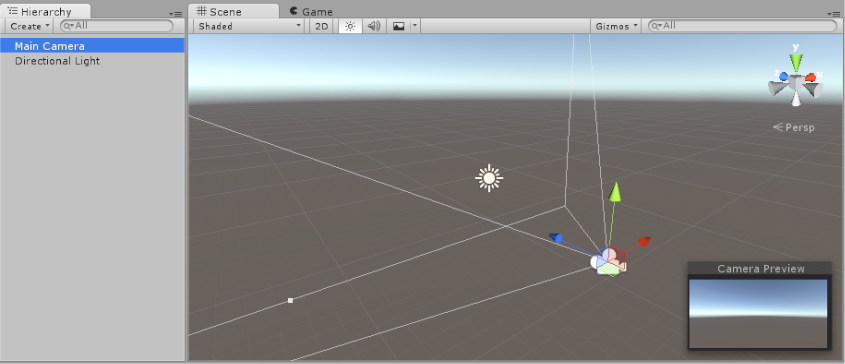
\includegraphics[width=\linewidth]{scene.jpg}
  \caption{Uma scene como apresentada no editor do Unity.}
  \label{fig:scene1}
\end{figure}
\subsection{Game Objects}

Game Objects ~\ref{fig:objects} são os objetos fundamentais no Unity que representam personagens, adereços e cenários, todos objetos de um jogo Unity são Game Objects. Game Objects não apresentam nenhuma funcionalidade própria, mas são containers para Componentes que dão funcionalidade e propriedades a um Game Object.

\begin{figure}[h!]
  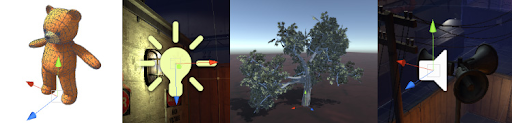
\includegraphics[width=\linewidth]{object.jpg}
  \caption{Objects representados no editor do Unity.}
  \label{fig:objects}
\end{figure}

Dependendo do tipo de Game Object que se deseja criar no Unity, se deve utilizar uma combinação diferente de componentes ~\ref{fig:objprop}. O Unity apresenta vários tipos de componentes pré-programados, mas é possível se criar novos utilizando a API de script do Unity em C\#.
\begin{figure}
  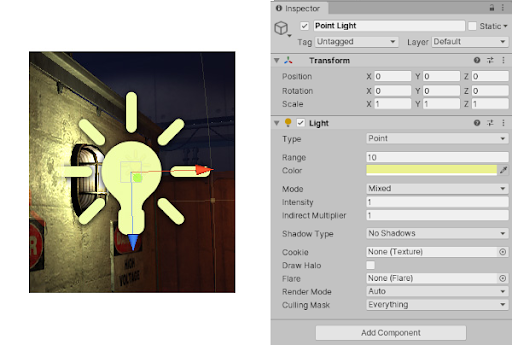
\includegraphics[width=\linewidth, scale = 0.2]{objprop.jpg}
  \caption{Objeto e seu menu de componentes.}
  \label{fig:objprop}
\end{figure}
\pagebreak
\subsection{Prefabs}

O sistema de Prefabs permite que o desenvolvedor crie, configure e armazene Game Objects completos com todos seus componentes, propriedades e gameObjects acoplados como um asset reutilizável. O Prefab ~\ref{fig:prefab} age como um template com o qual o desenvolvedor pode criar novas instâncias dentro de uma Scene.

	O sistema de Prefabs é melhor utilizado quando se precisa utilizar o mesmo GameObject múltiplas vezes dentro de uma Scene, ou em múltiplas Scenes dentro de um projeto, pois o uso de Prefabs permite que sejam feitas modificações síncronas em todas suas instâncias a partir de modificações no Prefab original.
	
	Qualquer modificação que se faz em um Prefab é automaticamente refletida em suas instâncias, mas modificações em instâncias do Prefab não afetam as outras instâncias ou o Prefab, possibilitando que as instâncias sejam customizadas de acordo com as necessidades.
	
	Outro utilidade importante de Prefabs é a instanciação de GameObjects em tempo de execução, o que pode ser utilizado para adicionar efeitos especiais, power ups, ou projéteis à Scene durante a execução do jogo.
\begin{figure}
  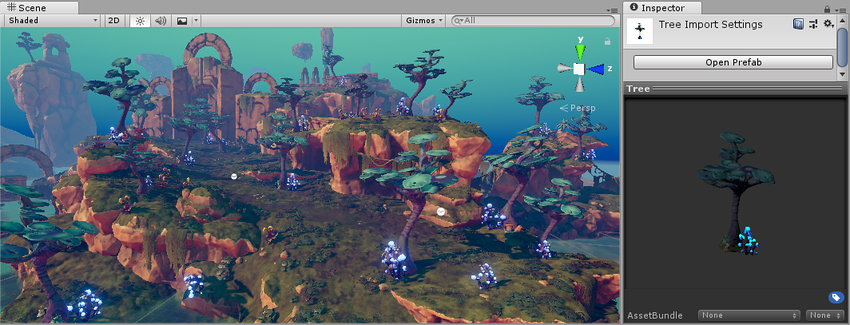
\includegraphics[width=\linewidth]{prefab.jpg}
  \caption{Uma prefab.}
  \label{fig:prefab}
\end{figure}	

\subsection{Scripts}

O Unity permite que sejam criados novos Componentes por meio de scripts em C\#, permitindo assim que o desenvolvedor modifique e adicione propriedades a GameObjects da maneira que desejar.

Um script se conecta ao funcionamento interno do Unity pela implementação de uma classe que deriva da classe interna chamada MonoBehaviour, o que permite que scripts sejam acopladas a GameObjects como Componentes.

\chapter{Estudo de Jogos Relevantes}

Neste capítulo serão apresentados as principais mecânicas básicas dos gêneros Coleção de Criaturas, \emph{RPG}, e a análise dos jogos que foram estudados como base para o desenvolvimento do projeto. 


\section{Mecânicas Relevantes}

As quatro mecânicas mais relevantes consideradas para a produção do projeto foram: Exploração de labirintos, encontros aleatórios, progressão por níveis e a captura de monstros, pois são as mecânicas que formam o pilar base para os jogos da franquia Pokémon e de outros RPGs similares.

	A mecânica de Exploração de Labirintos consiste em dividir cada área do jogo em diversos labirintos, onde o jogador deve atravessar para continuar o jogo. O fator diversão desse tipo de mecânica deriva da exploração do ambiente, da batalha contra inimigos encontrados pelo caminho, de descobrir segredos presentes nos labirintos e a sensação de conquista ao superar os obstáculos presentes no labirinto. 

	As batalhas em encontros aleatórios são obstáculos que os jogadores podem encontrar aleatoriamente ao se movimentar pelos ambientes do jogo. Durante os encontros aleatórios, jogadores precisam derrotar inimigos aleatórios para continuarem a progredir em direção ao objetivo principal. O fator diversão desta mecânica deriva da satisfação de ganhar uma batalha, e das possíveis recompensas que podem ganhar ao superar cada batalha.

	A progressão de força se refere a capacidade do jogador de se tornar mais forte durante o jogo, geralmente por meio de aquisição de recursos como equipamentos melhores e itens, por meio de novas habilidades ou por melhoria dos atributos dos personagens jogáveis. 

	A captura de monstros é a mecânica que permite que o jogador capture criaturas para utilizá-las para progredir no jogo.

\section{Séries de Jogos Estudas}

Durante esta seção será apresentado uma breve análise dos jogos estudados com o funcionamento das principais mecânicas de jogos que foram escolhidos para análises. Uma explicação mais profunda destas mecânicas serão apresentadas durante o capítulo 5, onde as análises foram fundamentais para a implementação do jogo.

\subsection{Pokémon}

Pokémon ~\cite{Pkmn} é a franquia de jogos mais bem sucedida da história, com mais de 90 bilhões de dólares arrecadados em vendas, seus jogos se destacam por serem acessíveis, fáceis de aprender, e terem um forte apelo ao público infantil.

Na maioria dos jogos \emph{mainline} de Pokémon a exploração do mundo é feita por meio de uma perspectiva \emph{top-down} ~\ref{fig:pokemon}, uma perspectiva onde o jogador enxerga o mundo de um ponto de vista acima do personagem que controla. No mundo explorável do jogo, o jogador pode descobrir novas áreas, segredos, itens espalhados, além de poder entrar em batalhas contra pokémons selvagens ou treinadores pokémons espalhados.

\begin{figure}[h!]
  \centering
  \begin{subfigure}[b]{0.49\linewidth}
    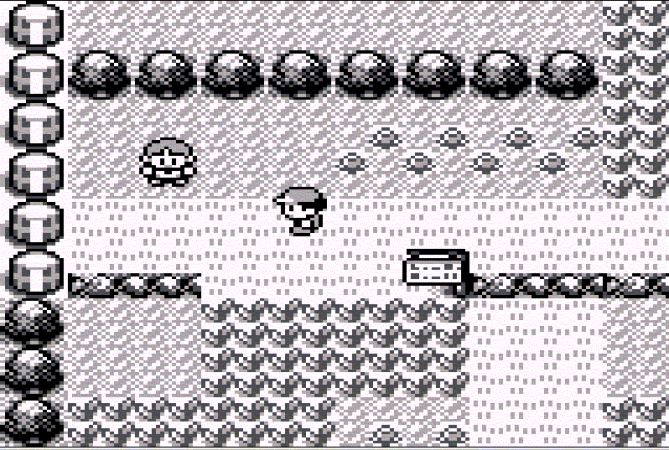
\includegraphics[width=\linewidth]{red.jpg}
     \caption{Pokémon Red - 1996.}
  \end{subfigure}
  \begin{subfigure}[b]{0.49\linewidth}
    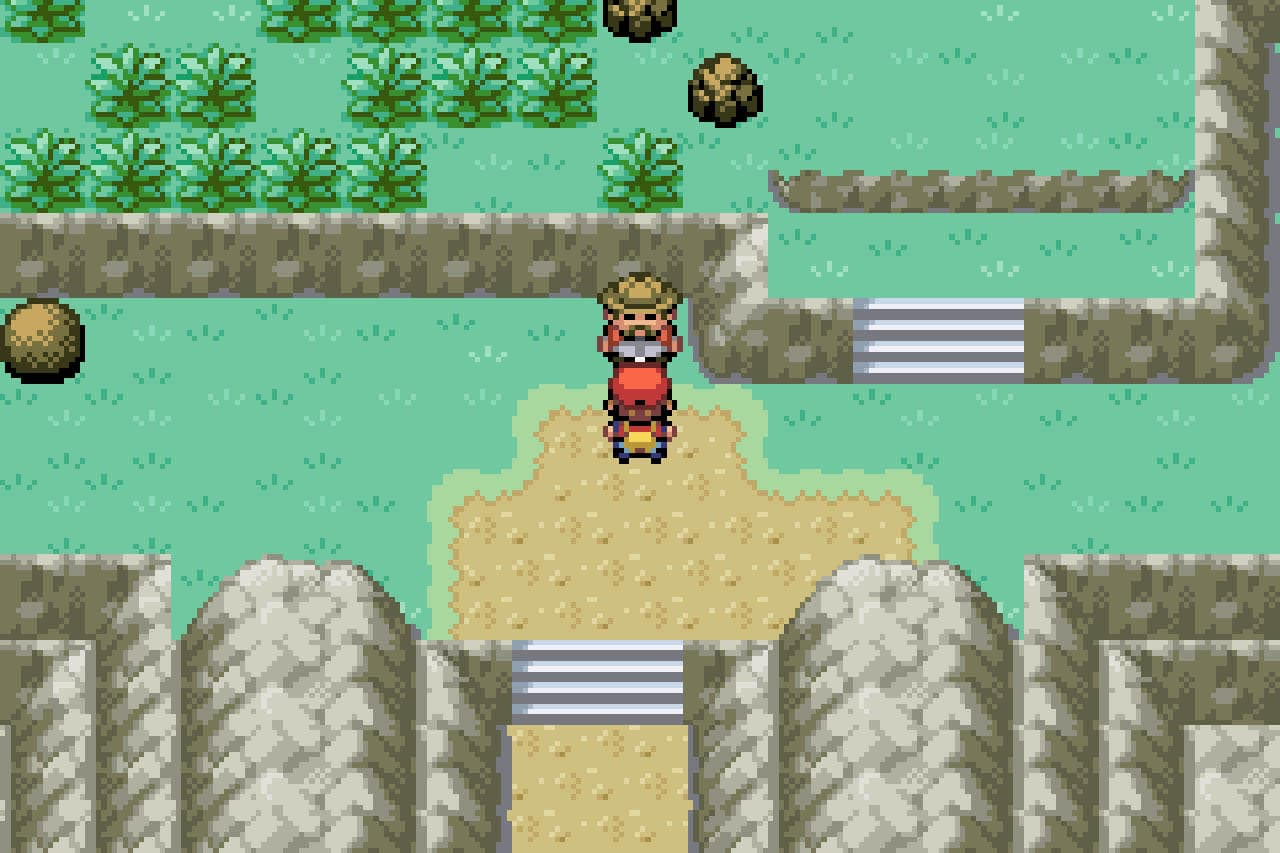
\includegraphics[width=\linewidth]{firered.jpg}
    \caption{Pokémon Fire Red - 2004.}
  \end{subfigure}
  \begin{subfigure}[b]{0.49\linewidth}
    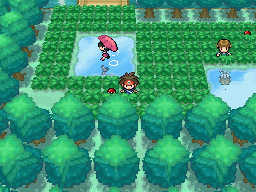
\includegraphics[width=\linewidth]{bw.jpg}
    \caption{Pokémon Black \& White - 2011.}
  \end{subfigure}
  \begin{subfigure}[b]{0.49\linewidth}
    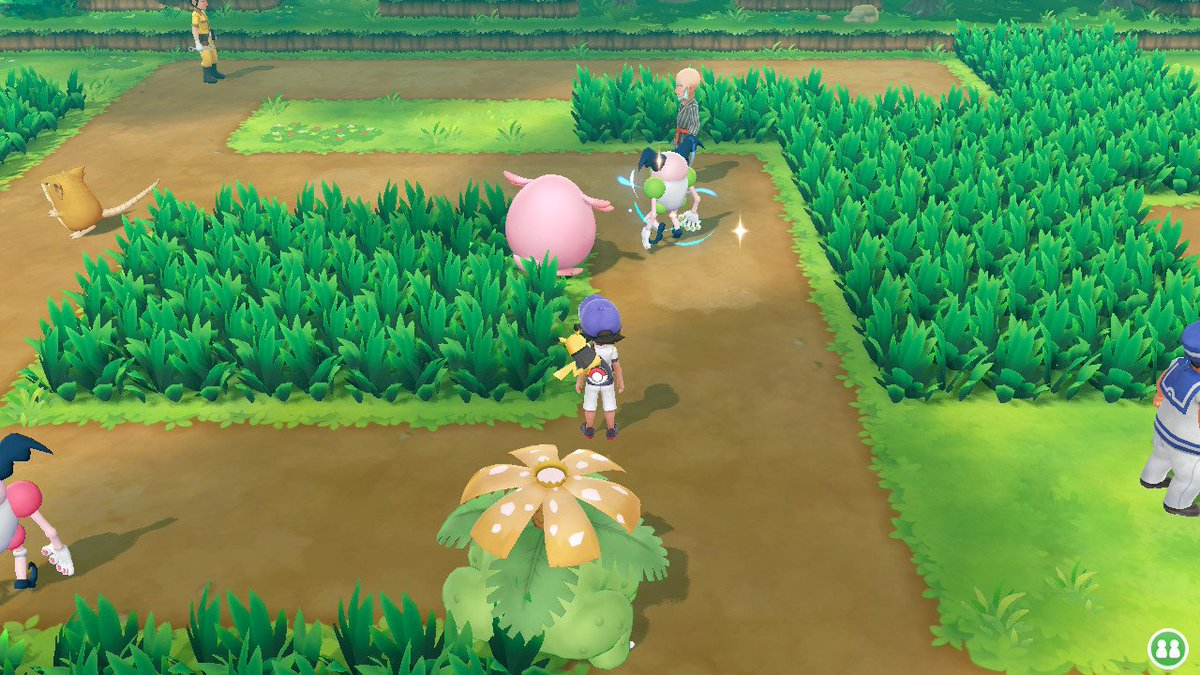
\includegraphics[width=\linewidth]{lgpikachu.jpg}
    \caption{Pokémon Let’s Go Pikachu - 2018.}
  \end{subfigure}
  \caption{Evolução da visão do mundo em Pokémon durante os anos.}
  \label{fig:pokemon}
\end{figure}

Este tipo de exploração de mundo é simples de se desenvolver, fácil para jogadores se entenderem e se localizarem, porém a imersão dentro do mundo do jogo pode ser mais rasa para alguns jogadores.

	As batalhas em pokémon ~\ref{fig:pokemon2} podem ocorrer de várias maneiras durante a exploração do mundo, sendo que o tipo mais comum é contra Pokémons selvagens encontrados randomicamente durante a exploração do mundo.

	Batalhas normalmente ocorrem no formato 1 contra 1, onde um dos pokémons do jogador troca turnos com um dos pokémons adversários até que os \emph{Hit Points} ou \emph{HP} de um deles cheguem a zero.

\begin{figure}[h!]
  \centering
  \begin{subfigure}[b]{0.3\linewidth}
    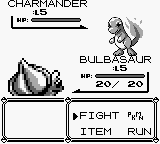
\includegraphics[width=\linewidth]{redb.jpg}
     \caption{Pokémon Red - 1996.}
  \end{subfigure}
  \begin{subfigure}[b]{0.4\linewidth}
    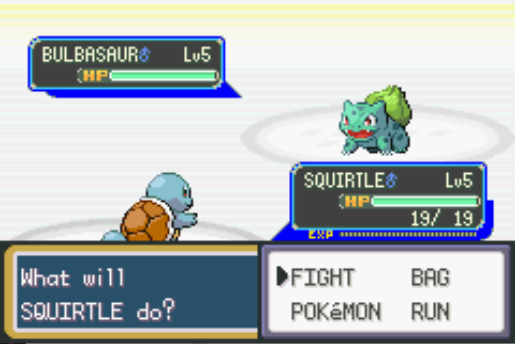
\includegraphics[width=\linewidth]{fireredb.jpg}
    \caption{Pokémon Fire Red - 2004.}
  \end{subfigure}
  \begin{subfigure}[b]{0.6\linewidth}
    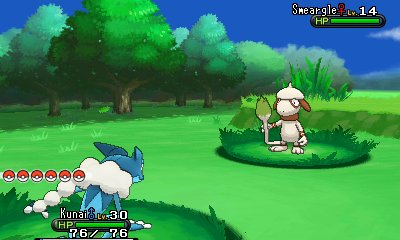
\includegraphics[width=\linewidth]{xyb.jpg}
    \caption{Pokémon XY - 2013.}
  \end{subfigure}
  \begin{subfigure}[b]{0.6\linewidth}
    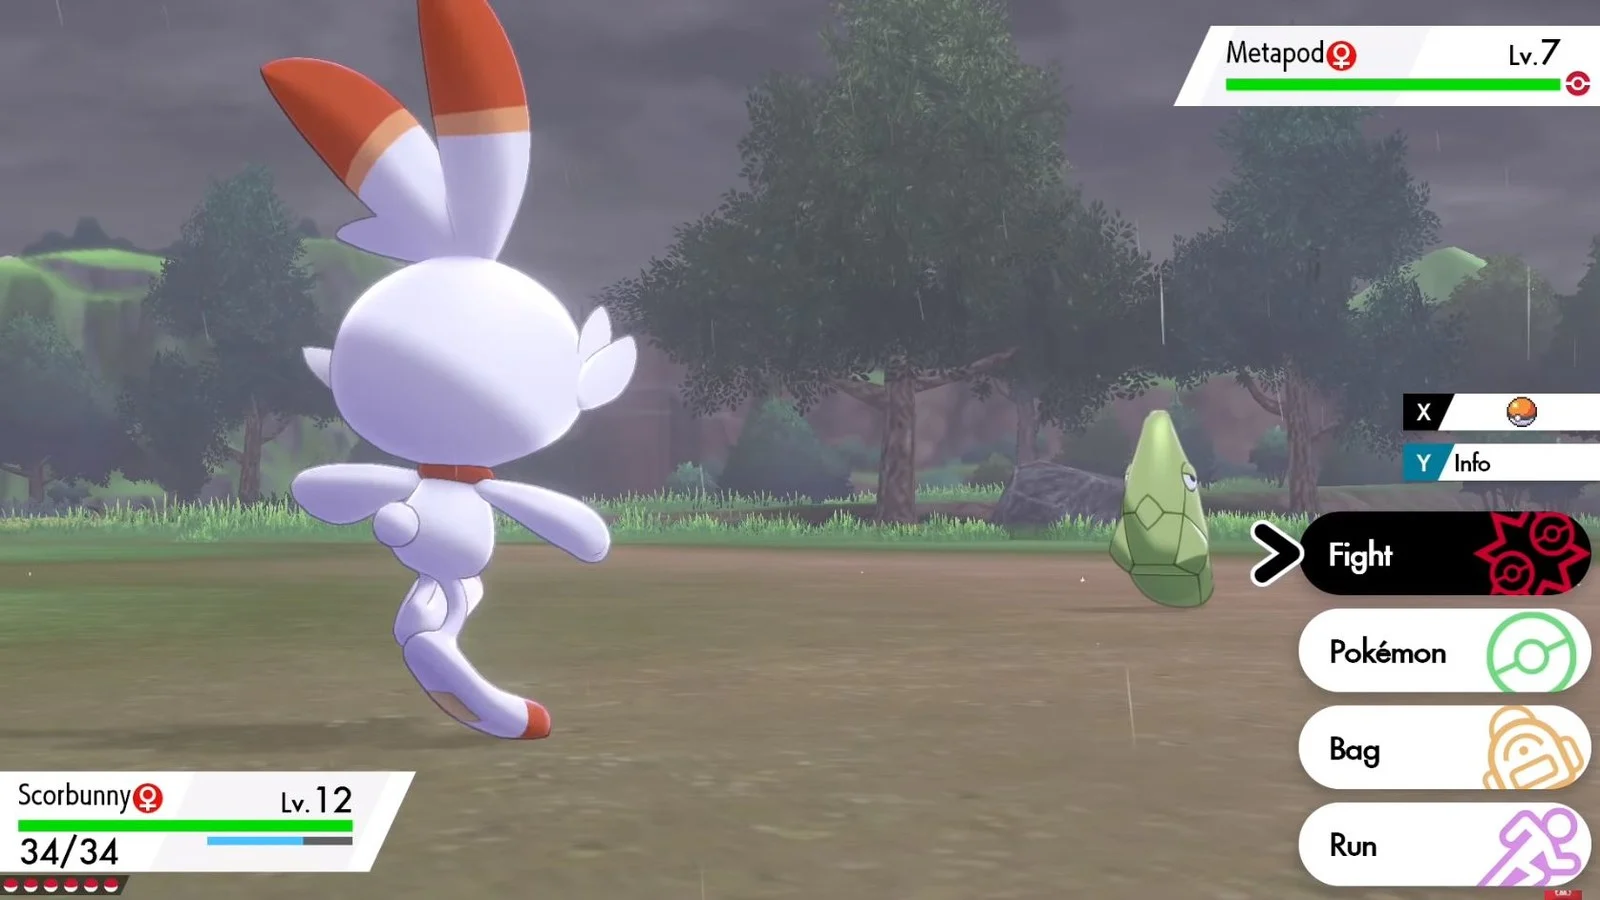
\includegraphics[width=\linewidth]{swsh.jpg}
    \caption{Pokémon Sword \& Shield - 2019.}
  \end{subfigure}
  \caption{Evolução das batalhas em Pokémon durante os anos.}
  \label{fig:pokemon2}
\end{figure}

O sistema de batalhas é simples e fácil de se aprender, possibilitando que até mesmo crianças que não saibam ler consigam se divertir com o jogo, ao mesmo tempo que apresenta mecânicas complexas e profundas, de modo que possa agradar fãs mais avançados. O problema deste modelo é que o design do jogo considera apenas os jogadores mais casuais da série, resultando em um jogo fácil onde não é necessário o uso eficiente das mecânicas de combate mais complexas e profundas que o jogo oferece.

\subsection{Shin Megami Tensei}

Shin Megami Tensei ~\cite{SMT}, também conhecidos pela sigla SMT, é uma franquia de jogos que, em sua maioria, consistem de jogos RPG de exploração de labirintos e negociação com demônios com os quais se podem fazer alianças para utilizá-los em batalhas.

	A exploração do mundo dos jogos SMT é feita de diferentes maneiras atualmente, mas esta análise se baseará nos jogos mais antigos, onde a exploração era feita por meio de exploração em primeira pessoa de diversos labirintos que formam cada pedaço do jogo ~\ref{fig:smt}, durante essa exploração jogadores podem encontrar itens, segredos, e demônios recrutáveis que podem ser utilizados para progredir dentro do jogo.

\begin{figure}[h!]
  \centering
  \begin{subfigure}[b]{0.4\linewidth}
    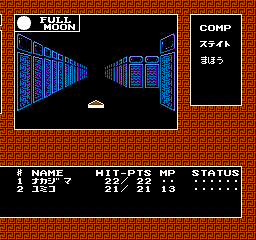
\includegraphics[width=\linewidth]{mt.jpg}
     \caption{Digital Devil Story: Megami Tensei - 1987.}
  \end{subfigure}
  \begin{subfigure}[b]{0.4\linewidth}
    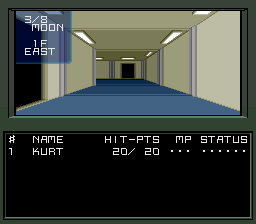
\includegraphics[width=\linewidth]{smt1.jpg}
    \caption{Shin Megami Tensei - 1992.}
  \end{subfigure}
  \begin{subfigure}[b]{0.4\linewidth}
    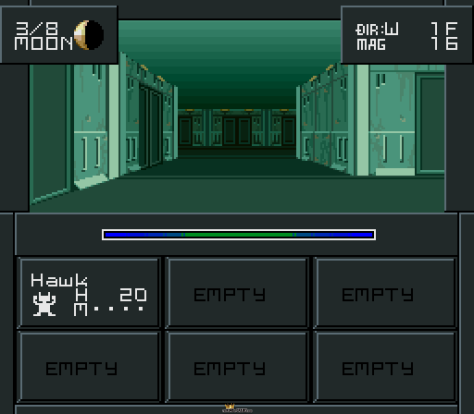
\includegraphics[width=\linewidth]{smt2.jpg}
    \caption{Shin Megami Tensei II - 1994.}
  \end{subfigure}
  \begin{subfigure}[b]{0.4\linewidth}
    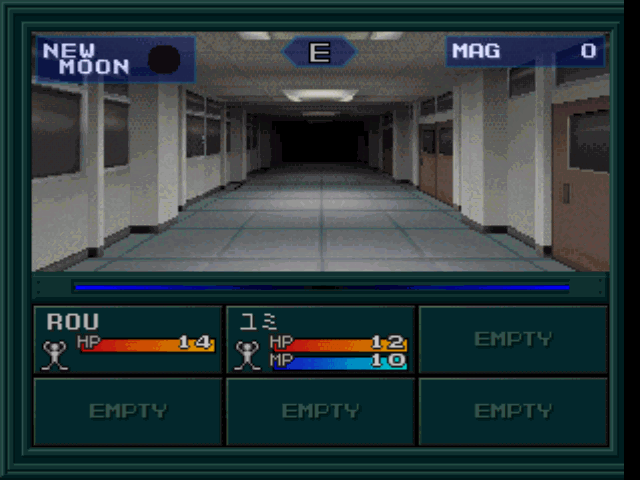
\includegraphics[width=\linewidth]{smtif.jpg}
    \caption{Shin Megami Tensei IF PS1 - 2002.}
  \end{subfigure}
  \caption{Exploração de mundo nos primeiros jogos da série Shin Megami Tensei.}
  \label{fig:smt}
\end{figure}

A exploração em primeira pessoa aumenta a imersão do jogador dentro do jogo, pode ser utilizada para criar uma sensação de maior claustrofobia, desorientação, e solidão, o que é utilizado para a criação da atmosfera e ambientação do jogo. A principal desvantagem deste tipo de exploração é a dificuldade de se localizar e a grande quantidade de batalhas que se deve enfrentar durante o percurso dos labirintos, o que pode se tornar uma atividade frustrante ao invés de recompensadora.

As batalhas em SMT ocorrem via encontros aleatórios durante a exploração de labirintos, o jogador deve utilizar seu grupo de aliados, podem ser ou não ser demônios, para derrotar os grupos de inimigos ~\ref{fig:smtb}. Durante o combate, o jogador tem a opção de negociar com demônios para que eles se tornem aliados.


\begin{figure}[h!]
  \centering
  \begin{subfigure}[b]{0.4\linewidth}
    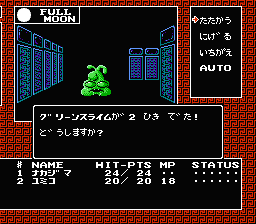
\includegraphics[width=\linewidth]{mtb.jpg}
     \caption{Digital Devil Story - 1987.}
  \end{subfigure}
  \begin{subfigure}[b]{0.4\linewidth}
    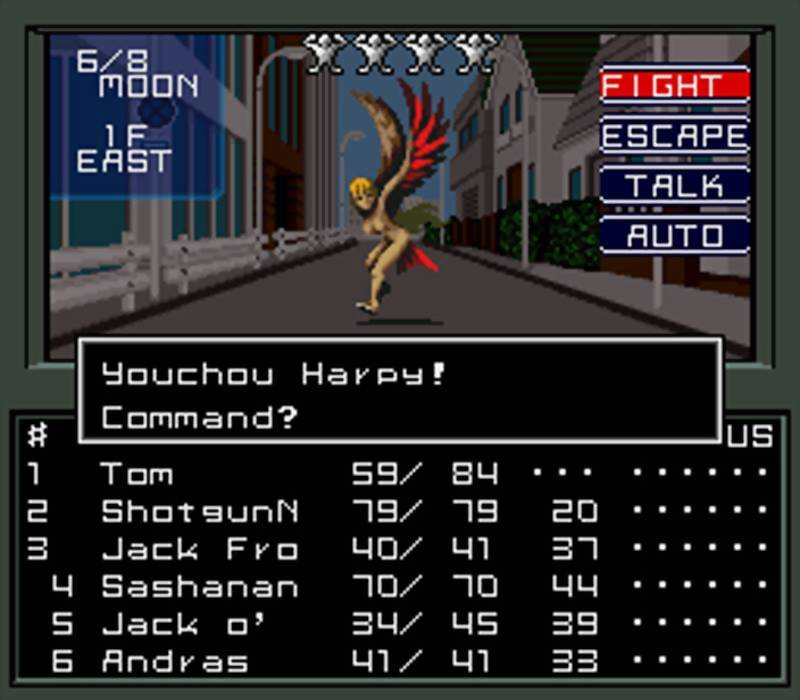
\includegraphics[width=\linewidth]{smt1b.jpg}
    \caption{Shin Megami Tensei - 1992.}
  \end{subfigure}
  \begin{subfigure}[b]{0.4\linewidth}
    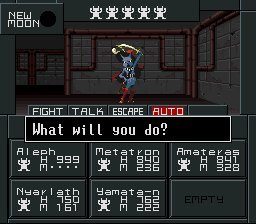
\includegraphics[width=\linewidth]{smt2b.jpg}
    \caption{Shin Megami Tensei II - 1994.}
  \end{subfigure}
  \begin{subfigure}[b]{0.4\linewidth}
    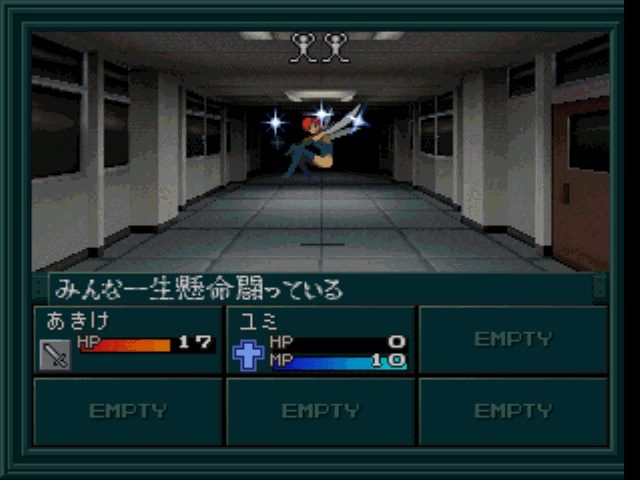
\includegraphics[width=\linewidth]{smtifb.jpg}
    \caption{Shin Megami Tensei IF PS1 - 2002.}
  \end{subfigure}
  \caption{Batalhas nos primeiros jogos da série Shin Megami Tensei.}
  \label{fig:smtb}
\end{figure}

O sistema de batalhas dos jogos SMT é bem complexo, com várias opções para o jogador utilizar estrategicamente e derrotar os diversos demônios e inimigos encontrados durante o jogo. A alta dificuldade das batalhas do jogo requer que o jogador utilize de todos os recursos disponíveis de maneira eficiente para progredir, tornando assim muito satisfatório e divertido a aprendizagem e eventual maestria do sistema de combate. A desvantagem deste modelo de batalhas é a necessidade do jogador dedicar tempo para entender todos os sistemas presentes, o que pode ser desencorajador para muitos jogadores mais casuais.

\subsection{Etrian Odyssey}

Etrian Odyssey ~\cite{EOW} é uma série de jogos de RPGs de exploração de labirintos desenvolvido pela Atlus, a mesma desenvolvedora da série de jogos Shin Megami Tensei, apresenta uma jogabilidade semelhante à série SMT mas com um foco bem maior em exploração de ambientes.

	A exploração do mundo em Etrian Odyssey é um dos principais focos do jogos, o jogador se move por labirintos com diversas temas diferentes, devendo criar seus próprios mapas por meio da tela touchscreen do Nintendo DS, e durante a exploração o jogador pode encontrar com diversos monstros, armadilhas, atalhos, itens, chefes e eventos especiais ~\ref{fig:eo}.

\begin{figure}[h!]
  \centering
  \begin{subfigure}[b]{0.36\linewidth}
    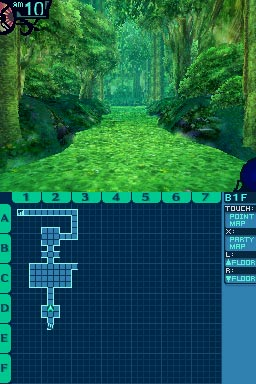
\includegraphics[width=\linewidth]{eo.jpg}
     \caption{Etrian Odyssey - 2007.}
  \end{subfigure}
  \begin{subfigure}[b]{0.44\linewidth}
    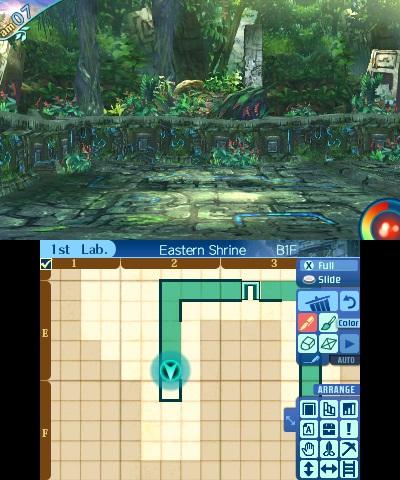
\includegraphics[width=\linewidth]{eonexus.jpg}
    \caption{Etrian Odyssey Nexus - 2018.}
  \end{subfigure}
  \caption{Evolução da exploração de mundo em Etrian Odyssey.}
  \label{fig:eo}
\end{figure}

As batalhas em Etrian Odyssey podem ocorrer por meio de encontros aleatórios durante a exploração do ambiente, ou por interação direta com monstros presentes nos labirintos ~\ref{fig:eob}. O jogo usa um sistema de classes semelhante aos presentes em RPGs de mesa tradicionais, onde o jogador deve montar um time de até 5 personagens, cada um com uma especialidade e habilidades diferentes. O sistema do jogo permite que o jogador crie cada personagem de maneira independente de forma que o time tenha as capacidades de ataque, defesa e suporte necessárias para conseguir derrotar todos os inimigos que encontrar em cada labirinto.

\begin{figure}[h!]
  \centering
  \begin{subfigure}[b]{0.36\linewidth}
    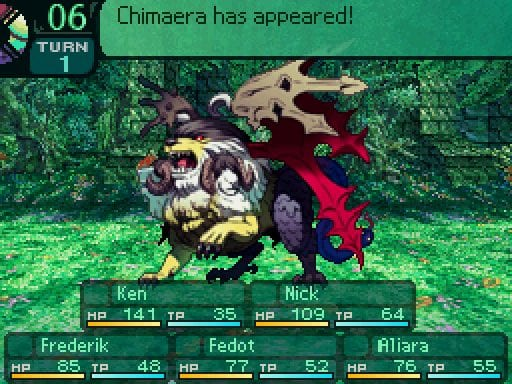
\includegraphics[width=\linewidth]{eob.jpg}
     \caption{Etrian Odyssey - 2007.}
  \end{subfigure}
  \begin{subfigure}[b]{0.44\linewidth}
    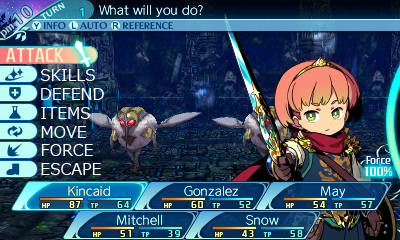
\includegraphics[width=\linewidth]{eonexusb.jpg}
    \caption{Etrian Odyssey Nexus - 2018.}
  \end{subfigure}
  \caption{Evolução das batalhas em Etrian Odyssey.}
  \label{fig:eob}
\end{figure}

\chapter{Design do Jogo}

O jogo foi dividido em duas partes principais, a exploração de labirintos, onde o jogador percorre o mundo em direção a um objetivo, e as batalhas por encontros aleatórios que podem ocorrer durante a exploração. Por meio do estudo dos jogos selecionados, o jogo foi desenvolvido implementando mecânicas desses diferentes jogos de maneira a criar o protótipo de um produto novo.

	Este capítulo é dedicado a uma visão geral de como foi feito o design do jogo e de como cada mecânica presente no jogo funciona, detalhes de implementação e funcionamento das mecânicas serão apresentados no capítulo 5.

\section{Objetivos do Jogador}

Objetivos em jogos servem para focar o jogador em uma determinada tarefa, dão propósito ao jogador, e servem como uma forma de guiar a experiência do jogador, no caso do protótipo feito, o objetivo apresentado ao jogador no começo do jogo é simples, entregar um pacote dado ao jogador por um NPC (\emph{Non-Player Character}) na cidade inicial a um NPC em uma outra cidade, e para chegar nesta cidade o jogador deve atravessar uma floresta. Apesar de parecer um objetivo muito simples e genérico, a real motivação para o jogador continuar jogando é a curiosidade de descobrir novos ambientes, novos monstros para interagir, e novas habilidades.

	O objetivo inicial de entregar o pacote de uma cidade a outra se traduz em vários pequenos objetivos intermediários durante o jogo, tais como: ficar mais forte para progredir; conseguir novos aliados; encontrar o caminho pelo labirinto; encontrar itens úteis; e desenvolver estratégias para otimizar batalhas.

\section{Obstáculos}

Obstáculos em jogos são os elementos que desafiam o jogador, que testam sua capacidade de resolver problemas, e que testam a habilidade do jogador de usar os recursos presentes no jogo.

	Neste protótipo os obstáculos são os labirintos que representam o ambiente explorável do jogo, e as batalhas aleatórias contra inimigos encontrados durante a exploração do ambiente.

\subsection{Labirintos}

A escolha de se ter a exploração do mundo em forma de labirintos em primeira pessoa partiu da limitação de assets disponíveis para se criar um vasto mundo que fosse interessante para o jogador. O uso de labirintos semelhantes aos encontrados em Shin Megami Tensei e Etrian Odyssey permitiu que se fosse usado poucos assets visuais para se criar um mapa grande e interessante para os jogadores explorarem ~\ref{fig:jogo1}.

\begin{figure}[h!]
  \centering
  \begin{subfigure}[b]{0.4\linewidth}
    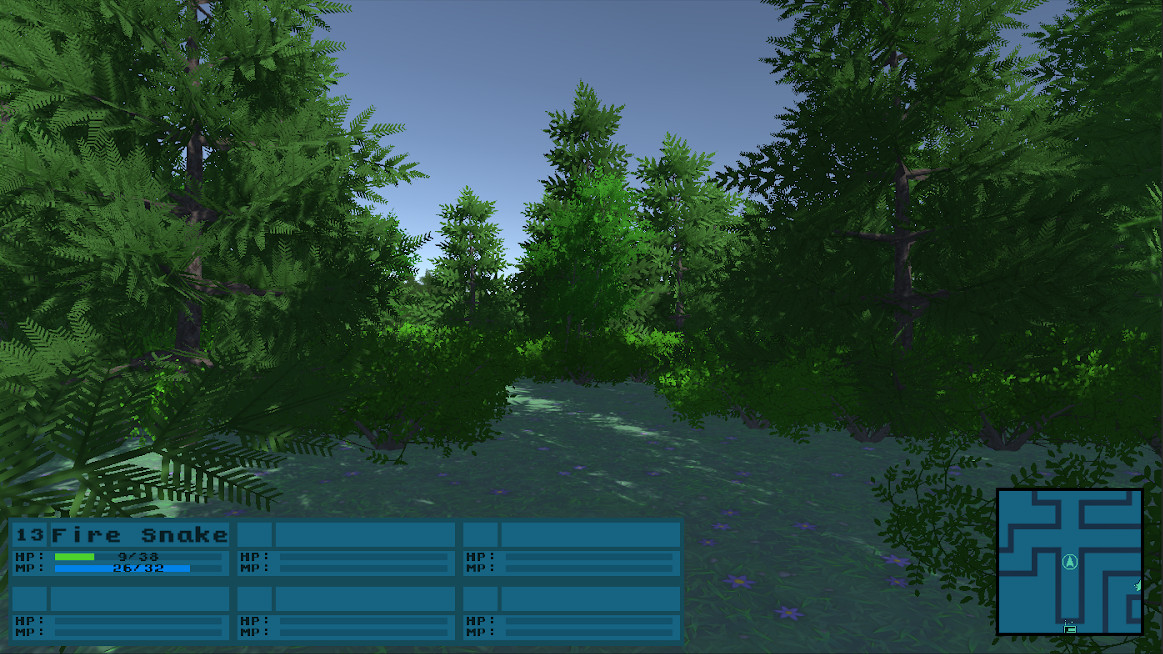
\includegraphics[width=\linewidth]{lab1.jpg}
  \end{subfigure}
  \begin{subfigure}[b]{0.4\linewidth}
    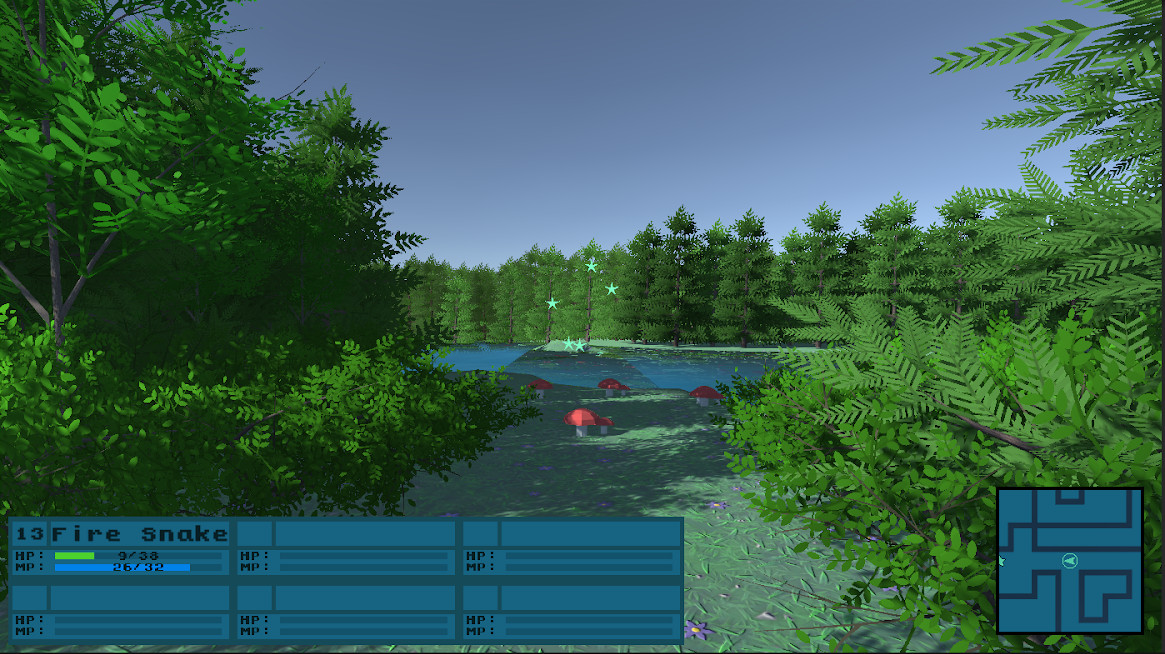
\includegraphics[width=\linewidth]{lab2.jpg}
  \end{subfigure}
  \caption{Etapa de exploração de labirintos.}
  \label{fig:jogo1}
\end{figure}

\subsubsection{Movimentação}

O jogador tem três opções de movimento: dar passos na direção da câmera, rotacionar em incrementos de 90° ao redor do eixo vertical, e passos para direita e esquerda.
A cada passo o que o jogador executa é incrementado um contador que decide se o jogador encontrou inimigos para iniciar uma batalha ou não.

\subsubsection{Menus}\label{owmenu}

Durante a exploração do labirinto o jogador pode abrir um Menu dividido em várias opções: \emph{Party} (Equipe), \emph{Bag} (Bolsa), \emph{Map} (Mapa), e Save ~\ref{fig:menu1}. Apenas as funcionalidades de \emph{Party} e \emph{Bag} foram implementadas por serem as relevantes ao funcionamento do protótipo.

\begin{figure}[h!]
  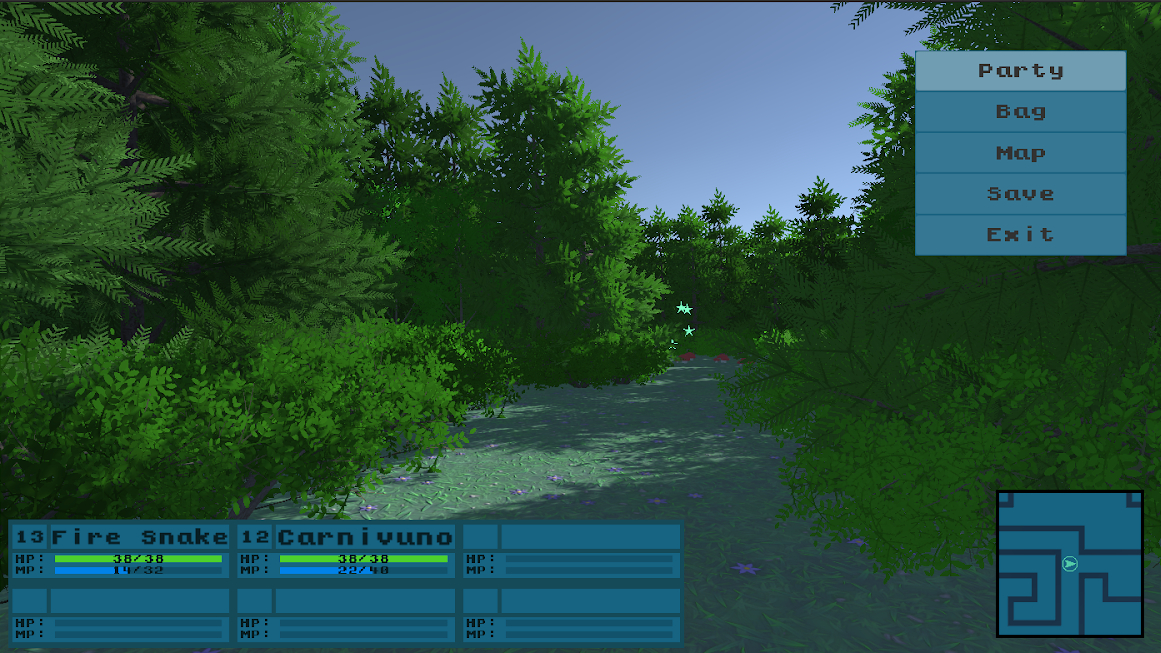
\includegraphics[width=\linewidth]{mainmenu.jpg}
  \caption{Main Menu aberto durante a exploração.}
  \label{fig:menu1}
\end{figure}

A opção \emph{Party} permite que o jogador veja informações dos demônios em seu grupo atual e os selecione para executar ações por meio de um novo menu que permite executar ações com o demônio selecionado. Essas ações são: Dar apelido ao demônio; Trocá-lo de posição no grupo; e utilizar habilidades ~\ref{fig:menu2}.

A opção Bag permite que o jogador use e veja informações sobre os itens que adquirir durante o jogo, uma caixa de mensagem é aberta e apresenta as informações do item atualmente selecionado.

\begin{figure}[h!]
  \centering
  \begin{subfigure}[b]{0.45\linewidth}
    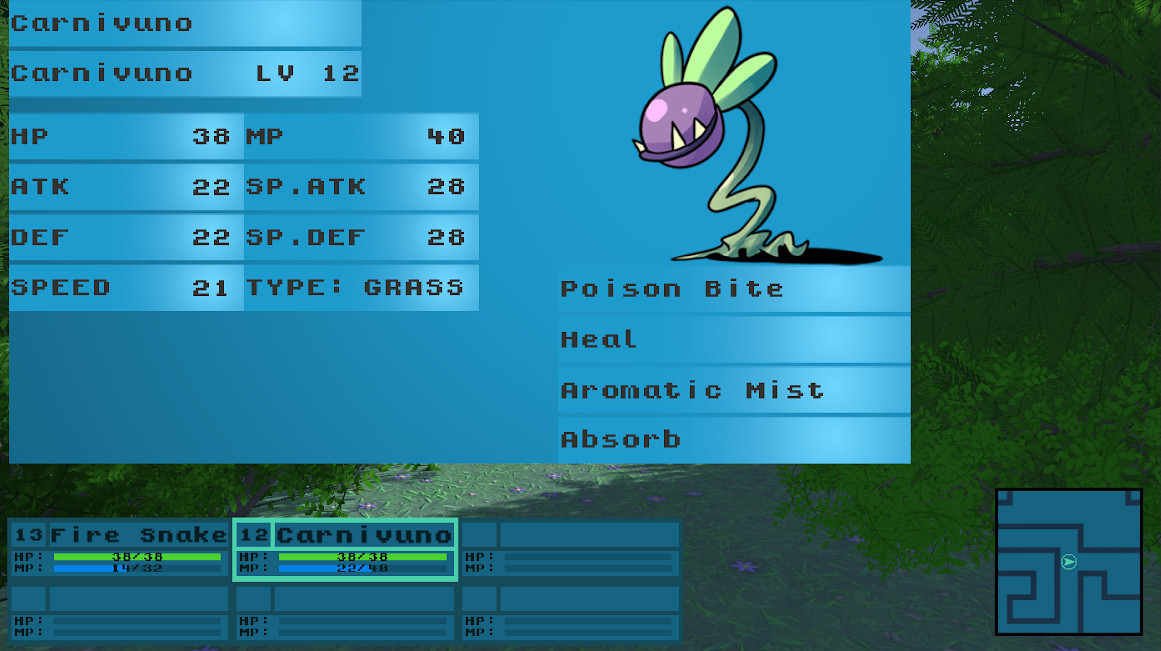
\includegraphics[width=\linewidth]{status.jpg}
     \caption{O jogador escolhe entre um dos membros da equipe após selecionar "Party".}
  \end{subfigure}
  \begin{subfigure}[b]{0.45\linewidth}
    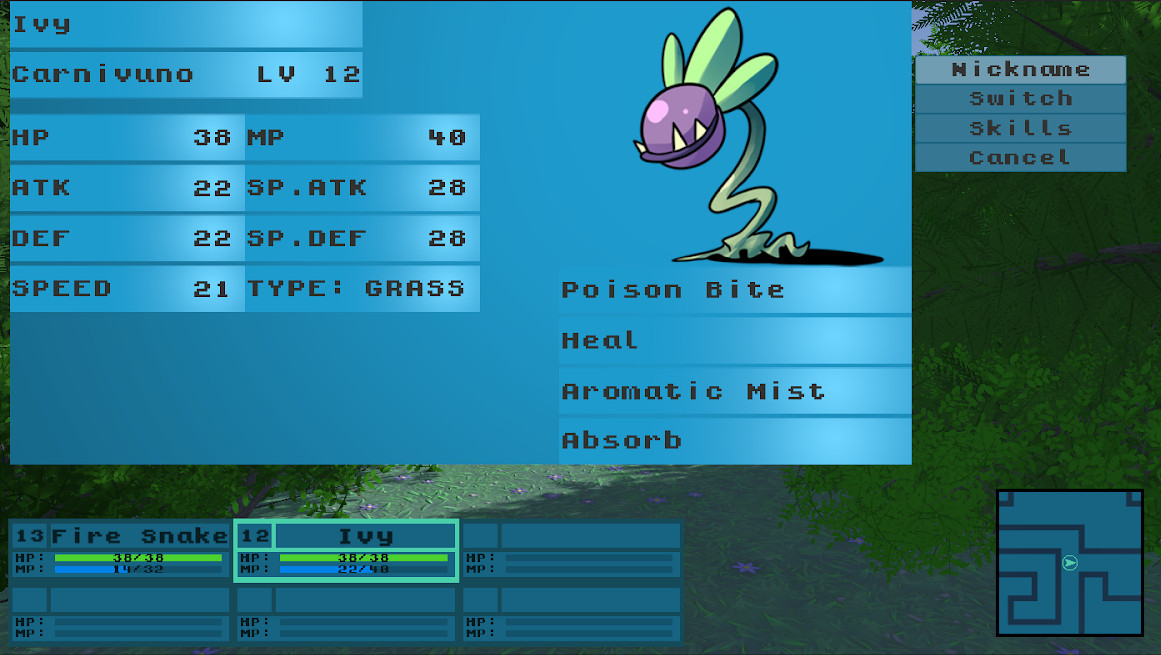
\includegraphics[width=\linewidth]{nickname.jpg}
    \caption{Um submenu de ações do personagem escolhido.}
  \end{subfigure}
  \begin{subfigure}[b]{0.45\linewidth}
    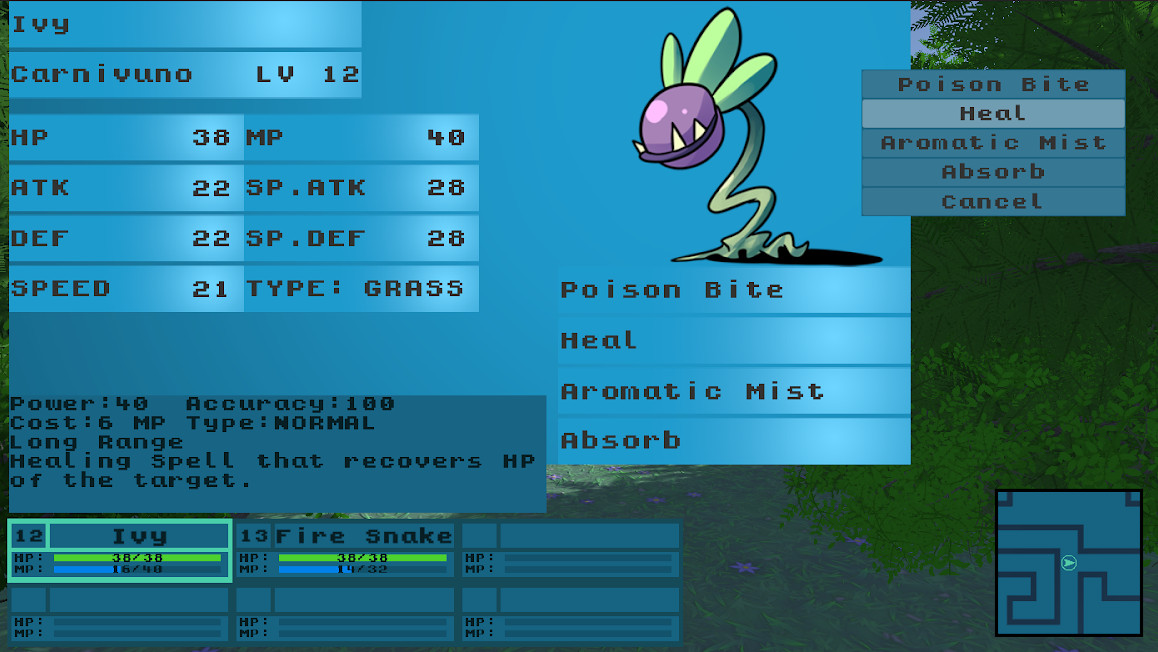
\includegraphics[width=\linewidth]{skills.jpg}
    \caption{SubMenu de \emph{skills} do personagem.}
  \end{subfigure}
  \begin{subfigure}[b]{0.45\linewidth}
    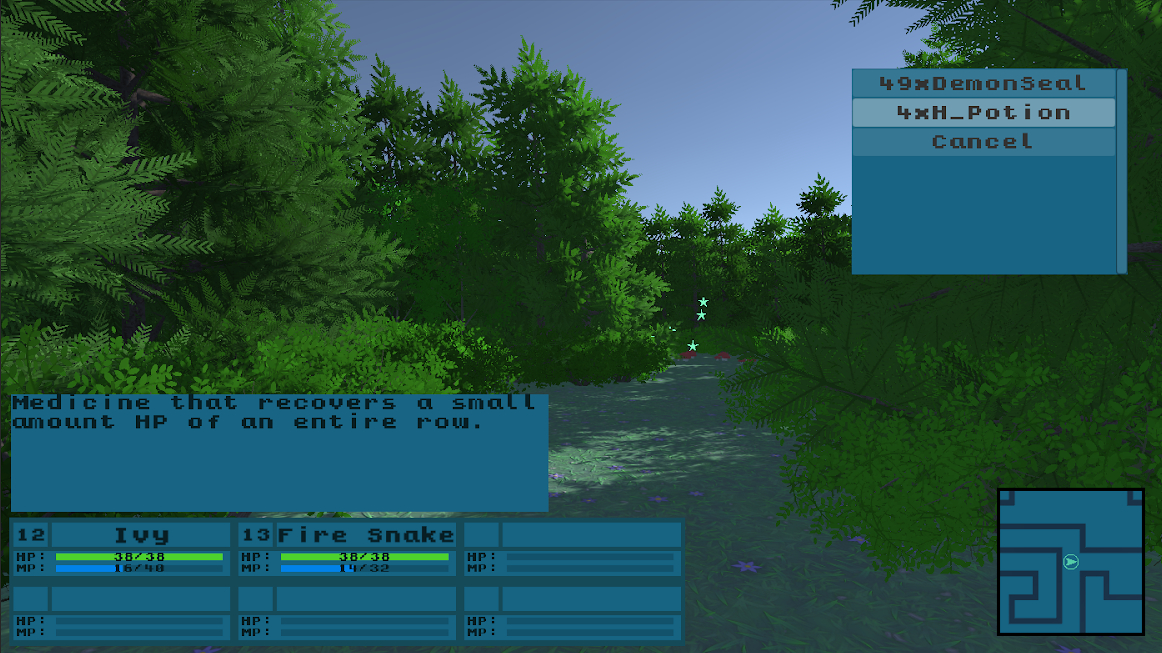
\includegraphics[width=\linewidth]{bag.jpg}
    \caption{Um submenu de ações é aberto após a escolha de "Bag".}
  \end{subfigure}
  \caption{SubMenu Bag de ações contendo os itens adquiridos.}
  \label{fig:menu2}
\end{figure}
\pagebreak
\subsubsection{Objetos Interativos}\label{chap:interactables}

Para deixar a exploração dos labirintos mais interessante e recompensadora para o jogador, foram criados objetos com os quais o jogador pode encontrar e interagir dentro dos labirintos.

	Itens podem ser encontrados espalhados pelo labirinto ~\ref{{fig:item1}}, indicados por partículas que saem do chão e por um ícone presente no minimapa no canto inferior direito. Partículas foram escolhidas para indicar a localização de itens devido a limitação de \emph{assets} disponíveis.
	
\begin{figure}[h!]
  \centering
  \begin{subfigure}[b]{0.4\linewidth}
    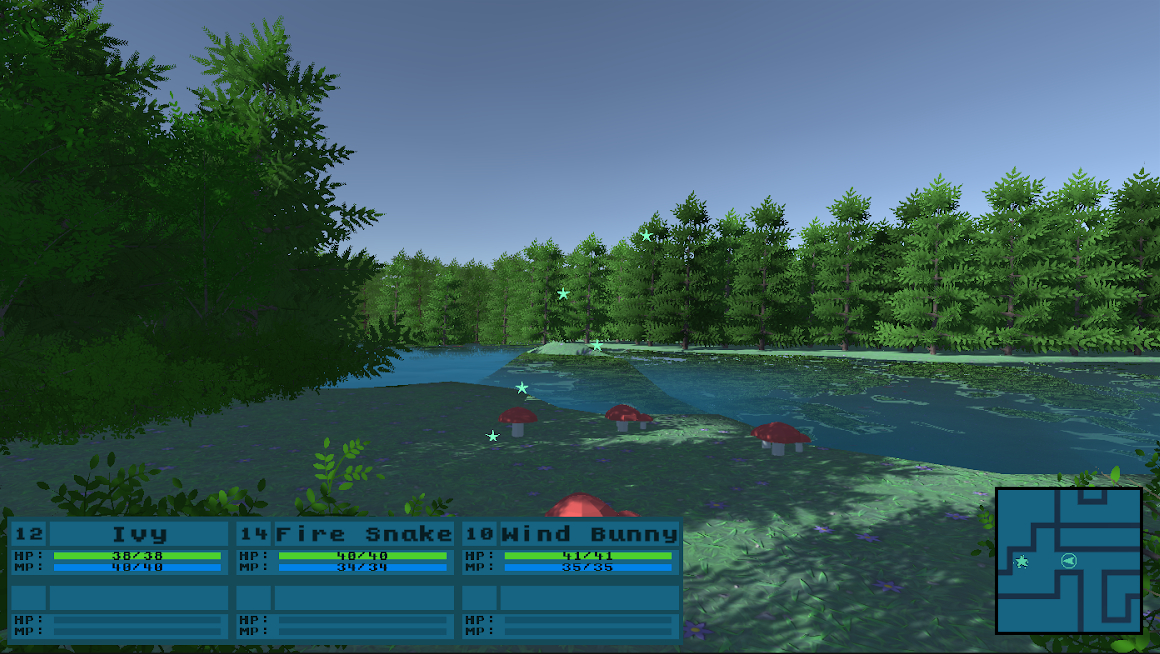
\includegraphics[width=\linewidth]{itemspot.jpg}
    \caption{Estrelas representam a localização de itens coletáveis.}
  \end{subfigure}
  \begin{subfigure}[b]{0.4\linewidth}
    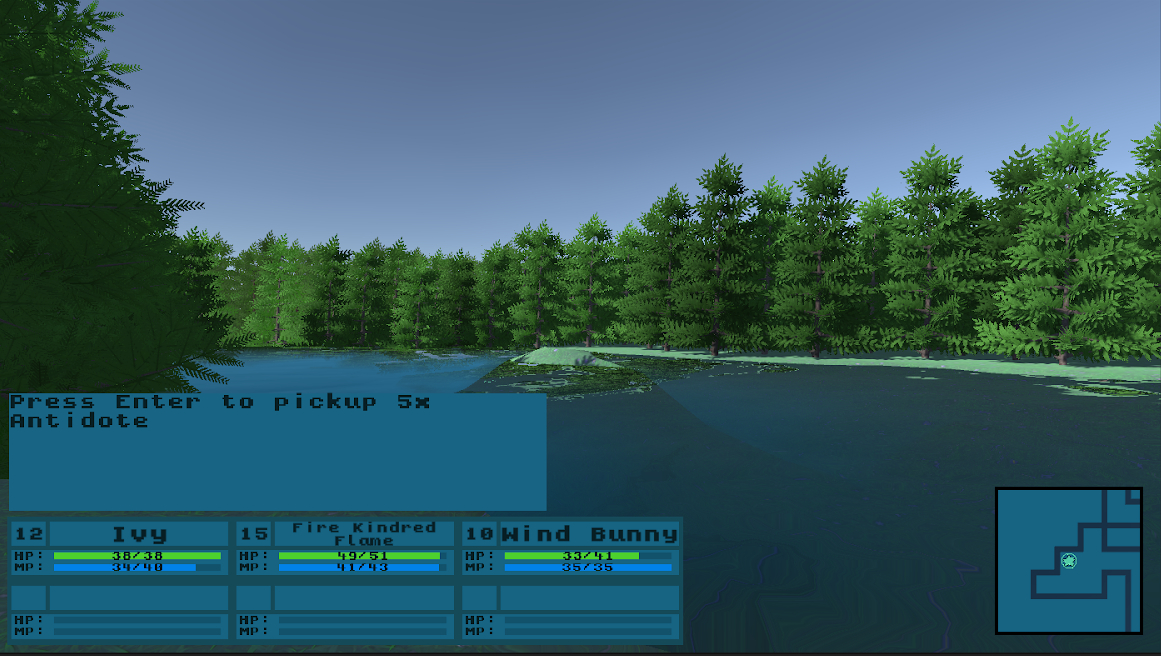
\includegraphics[width=\linewidth]{itemprompt.jpg}
    \caption{Uma caixa de mensagem é aberta ao se pisar sobre o item.}
  \end{subfigure}
  \caption{Representação de itens espalhados dentro do labirinto.}
  \label{fig:item1}
\end{figure}

Em jogos que apresentam ambientes em forma de labirintos e requerem que o jogador volte ao começo do labirinto como ocorre em jogos das franquias \emph{Etrian Odyssey} e \emph{Dark Souls}, o jogo garante que o jogador possa liberar atalhos para alcançar as áreas previamente alcançadas de maneira mais rápida e fácil, garantindo assim que o jogador não perca o sentimento de progresso mesmo que precise voltar ao começo do labirinto. Por essa razão foram criados atalhos semelhantes aos encontrados em \emph{Etrian Odyssey}, que permitem que o jogador atravesse paredes do labirinto.

	Os atalhos começam permitindo a passagem apenas por um dos lados da parede, mas após serem utilizados pelo menos 1 vezes, eles passam a permitir a travessia por ambos os lados da parede. Os atalhos devem ser algo que o jogador deve procurar ativamente, assim por design os locais com atalho são indicados apenas por pequenos indicadores visuais (como colônias de cogumelo crescendo juntos) ~\ref{fig:shortcut}, ou pelo próprio design do labirinto em si.

\begin{figure}[h!]
  \centering
  \begin{subfigure}[b]{0.47\linewidth}
    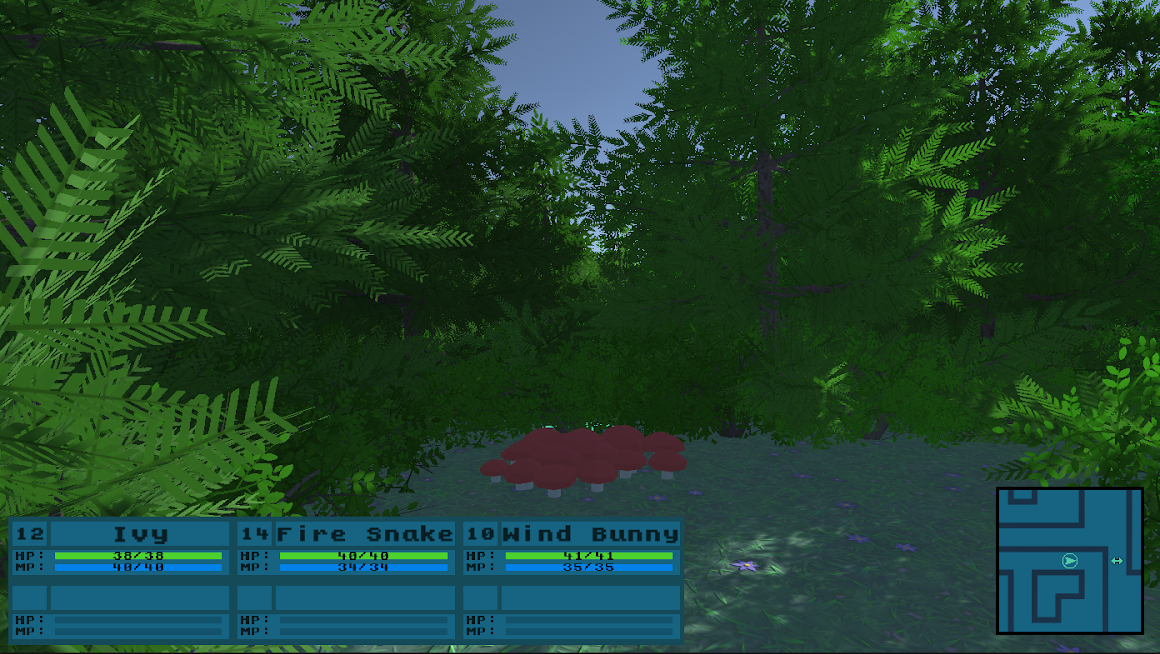
\includegraphics[width=\linewidth]{cogumelos.jpg}
     \caption{Conjunto de cogumelos dando a dica de que existe uma passagem.}
  \end{subfigure}
  \begin{subfigure}[b]{0.47\linewidth}
    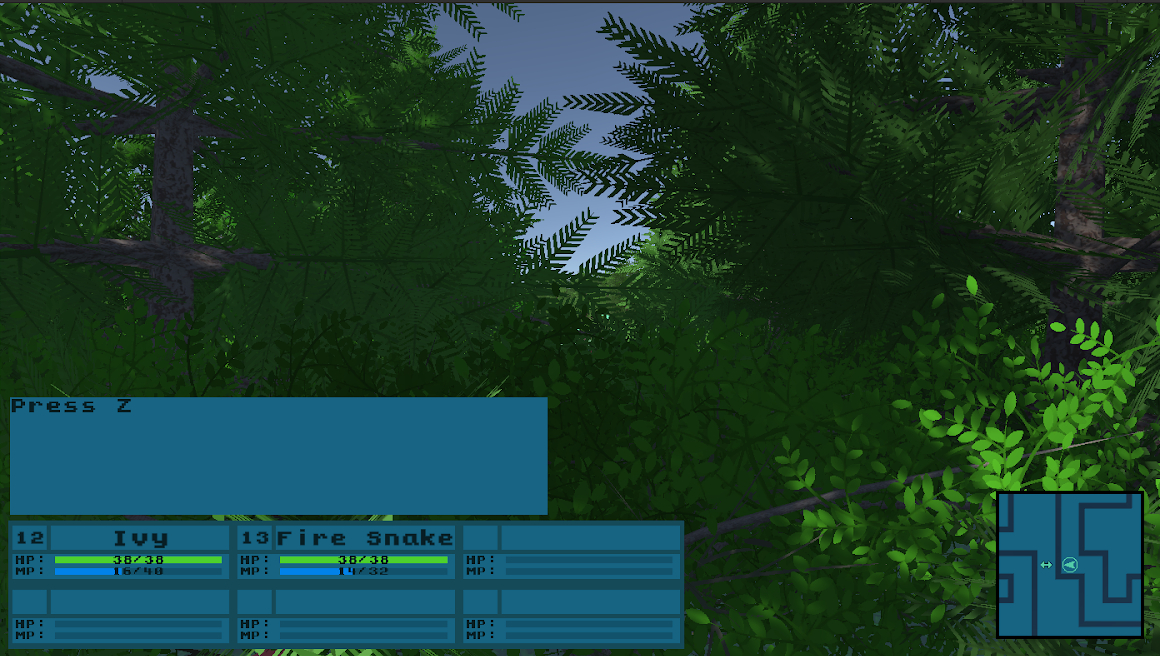
\includegraphics[width=\linewidth]{prompt.jpg}
    \caption{Caixa de diálogos se abre ao ficar de frente ao atalho.}
  \end{subfigure}
  \begin{subfigure}[b]{0.47\linewidth}
    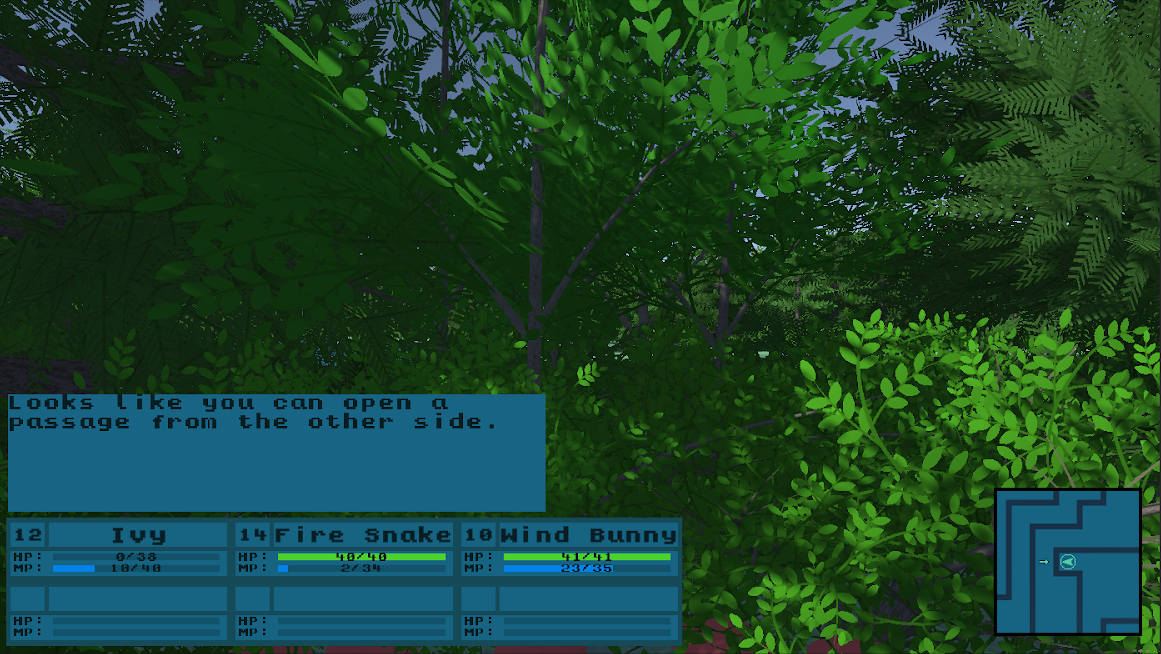
\includegraphics[width=\linewidth]{warning.jpg}
    \caption{Mensagem indica que é necessário se abrir caminho pelo outro lado.}
  \end{subfigure}
  \begin{subfigure}[b]{0.47\linewidth}
    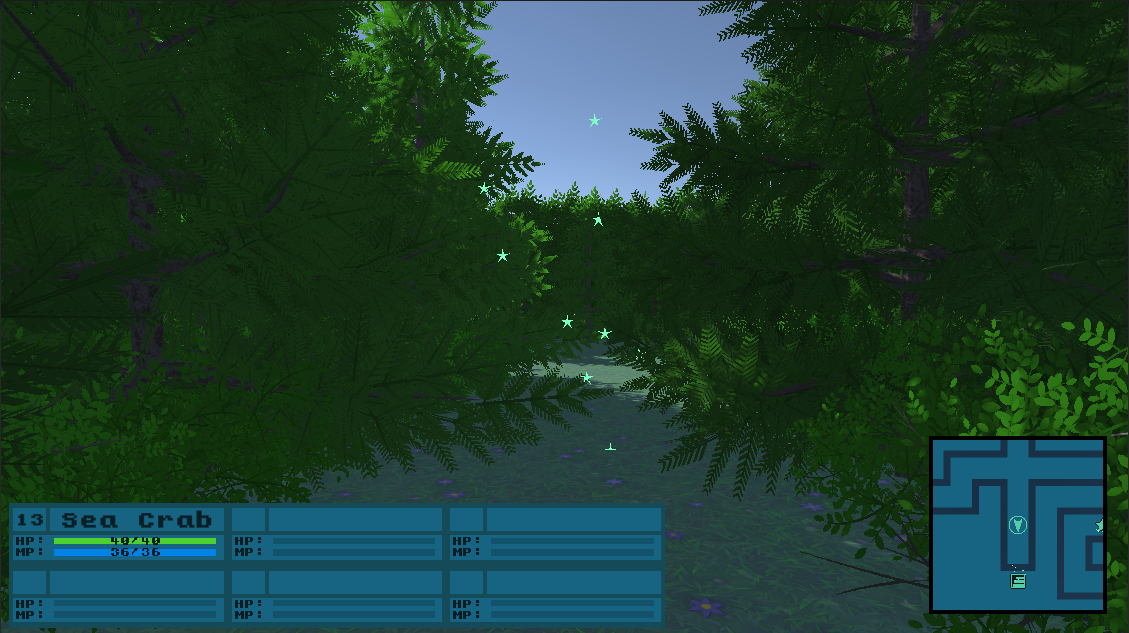
\includegraphics[width=\linewidth]{exit.jpg}
    \caption{A saída dos labirintos são indicadas por estrelas em frente a áreas vazias.}
  \end{subfigure}
  \caption{Interação com atalhos durante a exploração do labirinto.}
  \label{fig:shortcut}
\end{figure}
\pagebreak
\subsubsection{Mini-mapa}

A visão em primeira pessoa torná muito desorientador trafegar pelo labirinto portanto para melhorar a capacidade de localização durante a exploração dos labirintos, foi criado um mini mapa ~\ref{fig:minimapa1} que apresenta a visão superior do labirinto com ícones ~\ref{fig:minimapicons} que indicam objetos interativos e que não rotaciona junto com o jogador, permitindo que o jogador mais facilmente se localize e não fique andando em círculos, o que poderia se tornar um fator muito frustrante dentro do jogo.

\begin{figure}[h!]
 \centering
  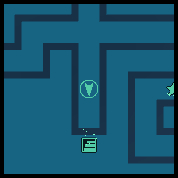
\includegraphics[width=0.4\linewidth]{minimap.jpg}
  \caption{O minimapa apresenta uma representação do labirinto visto de cima.}
  \label{fig:minimapa1}
\end{figure}

\begin{figure}[h!]
  \centering
  \begin{subfigure}[b]{0.1\linewidth}
    
\includegraphics[width=\linewidth]{icon1.jpg}
  \end{subfigure}
  \begin{subfigure}[b]{0.1\linewidth}
    
\includegraphics[width=\linewidth]{icon2.jpg}
  \end{subfigure}
  \begin{subfigure}[b]{0.1\linewidth}
    
\includegraphics[width=\linewidth]{icon3.jpg}
  \end{subfigure}
  \begin{subfigure}[b]{0.1\linewidth}
    
\includegraphics[width=\linewidth]{icon4.jpg}
  \end{subfigure}
  \begin{subfigure}[b]{0.1\linewidth}
    
\includegraphics[width=\linewidth]{playericon.png}
  \end{subfigure}
  \caption{Conjunto de Ícones presentes no minimapa.}
  \label{fig:minimapicons}
\end{figure}

\subsection{Batalhas}

Encontros aleatórios são uma mecânica que os videogames adotaram diretamente dos RPGs de mesa, onde ocasionalmente o DM (do inglês \emph{Dungeon Master}) jogava dados para determinar quando e quais inimigos o grupo de jogadores iria ter que enfrentar durante o jogo.

	Encontros aleatórios adiciona ao jogo um elemento de surpresa e mistério, onde o jogador nunca sabe quando e o que terá que enfrentar diante, e assim é capaz de invocar sentimentos de suspense, curiosidade, alívio e até medo. Esta mecânica também apresenta suas desvantagens, encontros aleatórios interrompem o fluxo de exploração do mundo e progresso dos jogadores podendo se tornar muito frustrantes, o que é um problema recorrente nos jogos mais antigos da série \emph{Shin Megami Tensei}. 

	O sistema de encontros aleatórios desenvolvido é semelhante ao encontrado em \emph{Etrian Odyssey}, que por apresentar um sistema onde o jogador deve dar um certo número de passos antes de encontrar uma batalha contra inimigos, possibilitando assim um fluxo mais natural e menos frustrante da exploração do labirinto. 

	As batalhas são em turnos divididos em duas partes: A escolha de ações, onde o jogador deve escolher estrategicamente as ações de cada um de seus personagens; e a etapa de batalha, onde as ações de todos os personagens em batalha são executadas por ordem de prioridade e velocidade. O sistema de batalha foi desenvolvido aplicando conceitos aprendidos ao estudar os sistemas de batalha encontrados em \emph{Shin Megami Tensei}, \emph{Etrian Odyssey}, e \emph{Pokémon}.

\subsubsection{Inimigos}

Os inimigos são encontrados aleatoriamente em grupos de 1 a 6 demônios, cada grupo de demônios é predefinido por uma tabela de encontros e são balanceados de acordo com as zonas em que são encontrados.

\subsubsection{Stats}\label{info:stats}

\emph{Stats} (do inglês \emph{Statistics}) são as características dos demônios que determinam sua força dentro do jogo.

\begin{itemize}
\item Level: Determina a força geral de um demônio, quanto maior o level de um demônio maior seus outros \emph{stats}.
\item HP: Sigla para \emph{Hit Point}, determina quanto dano um demônio pode receber antes de ficar incapacitado.
\item MP: Sigla para \emph{Mana Point}, são pontos que podem ser gastos para utilizar habilidades especiais em batalha.
\item ATK: O status de ataque, determina parcialmente o quanto de dano um demônio causa quando utiliza golpes de corpo a corpo.
\item DEF: O status de defesa, determina parcialmente o quanto de dano um demônio recebe de um golpe corpo a corpo.
\item SP.ATK: O status de ataque especial, determina parcialmente o quanto de dano um demônio causa quando utiliza golpes a distância.
\item SP.DEF: O status de defesa especial, determina parcialmente o quanto de dano um demônio recebe de um golpe a distância.
\item SPEED:  O status de velocidade, determina o ordem em que os demônios executam uma ação em batalha
\item TYPE: O tipo elemental do demônio, determina que habilidades pode aprender, e suas resistências e fraquezas contra habilidades de outros tipos elementais.
\end{itemize}

Um exemplo dos \emph{stats} de um demônio como são representados dentro do jogo pode ser visto na figura ~\ref{fig:stats}

\begin{figure}[h!]
 \centering
  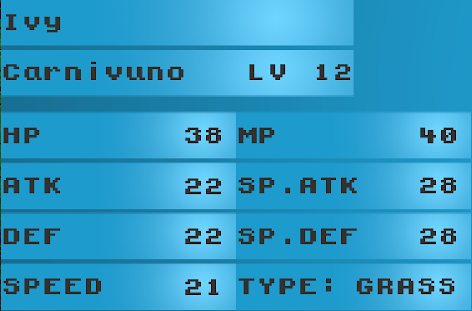
\includegraphics[width=0.5\linewidth]{statscreen.jpg}
  \caption{Os stats de um demônio como representados em jogo.}
  \label{fig:stats}
\end{figure}

\subsubsection{Types}

Uma das mecânicas mais comuns em jogos RPGs é a mecânica de existir diferentes tipos de ataques e habilidades como atributos diferentes e cada personagem dentro do jogo ter fraquezas e resistências a diferentes tipos de ataques. Em \emph{Dark Souls} o jogador pode utilizar uma grande variedade de armas e magias para atacar as fraquezas dos inimigos e causar dano adicional, e podem utilizar diferentes tipos de armadura para resistir a diferentes tipos de dano que inimigos podem causar a ele. Em \emph{Fire Emblem} cada tipo de unidade que o jogador controla durante as batalhas possuem suas respectivas resistências e fraquezas, dando ao jogador uma camada a mais de estratégia a ser considerada para posicionar suas unidades a fim de derrotar inimigos sem que perca suas próprias unidades. Em \emph{SMT} e \emph{Etrian Odyssey} cada monstro encontrado tem diferentes resistencias e  a diferentes tipos de armas e diferentes tipos de magia, forçando o jogador a criar uma equipe equilibrada a fim de conseguir enfrentar todos os desafios enfrentados durante o jogo. E por fim em Pokémon as resistências, fraquezas e ataques que cada pokémon pode aprender são todas definidas pelo seu tipo, que pode ser um ou dois de um total de 18 tipos diferentes.

Para este jogo foi utilizado um sistema de tipos semelhante ao encontrado em pokémon, pois torna a implementação da mecânica mais simples e fácil de ser desenvolvida, dado que ao invés de precisar determinar as resistências e fraquezas de cada demônio, é apenas necessário determina-las para cada tipo elemental.

Para o jogo temos 13 tipos diferentes com cada resistência e fraqueza definidas de acordo com a tabela \ref{resistance}, onde as linhas representam o tipo do ataque, e as colunas o tipo do demônio defensor, e os valores representam o multiplicador aplicado ao dano.

\begin{table}[!htp]\centering
\caption{Tabela de resistências.}\label{resistance}
\scriptsize
\begin{tabular}{lrrrrrrrrrrrrr}\toprule
ATK|DEF &NORMAL &FIRE &GRASS &WATER &AIR &DARK &LIGHT &ICE &ROCK &POISON &DRAGON &BUG \\\cmidrule{1-13}
NORMAL &1 &1 &1 &1 &1 &1 &1 &1 &\cellcolor[HTML]{e06666}0.5 &1 &1 &1 \\\cmidrule{1-13}
FIRE &1 &\cellcolor[HTML]{e06666}0.5 &\cellcolor[HTML]{00ff00}2 &\cellcolor[HTML]{e06666}0.5 &1 &1 &1 &\cellcolor[HTML]{00ff00}2 &\cellcolor[HTML]{e06666}0.5 &1 &\cellcolor[HTML]{e06666}0.5 &\cellcolor[HTML]{00ff00}2 \\\cmidrule{1-13}
GRASS &1 &\cellcolor[HTML]{e06666}0.5 &\cellcolor[HTML]{e06666}0.5 &\cellcolor[HTML]{00ff00}2 &1 &1 &1 &\cellcolor[HTML]{e06666}0.5 &\cellcolor[HTML]{00ff00}2 &\cellcolor[HTML]{e06666}0.5 &1 &\cellcolor[HTML]{e06666}0.5 \\\cmidrule{1-13}
WATER &1 &\cellcolor[HTML]{00ff00}2 &\cellcolor[HTML]{e06666}0.5 &\cellcolor[HTML]{e06666}0.5 &\cellcolor[HTML]{e06666}0.5 &1 &1 &\cellcolor[HTML]{e06666}0.5 &\cellcolor[HTML]{00ff00}2 &1 &\cellcolor[HTML]{e06666}0.5 &1 \\\cmidrule{1-13}
AIR &1 &1 &\cellcolor[HTML]{00ff00}2 &1 &1 &1 &1 &\cellcolor[HTML]{e06666}0.5 &\cellcolor[HTML]{e06666}0.5 &1 &\cellcolor[HTML]{e06666}0.5 &\cellcolor[HTML]{00ff00}2 \\\cmidrule{1-13}
DARK &\cellcolor[HTML]{00ff00}2 &1 &1 &1 &1 &\cellcolor[HTML]{e06666}0.5 &\cellcolor[HTML]{00ff00}2 &1 &1 &1 &\cellcolor[HTML]{00ff00}2 &\cellcolor[HTML]{e06666}0.5 \\\cmidrule{1-13}
LIGHT &1 &1 &1 &1 &1 &\cellcolor[HTML]{00ff00}2 &\cellcolor[HTML]{e06666}0.5 &1 &1 &\cellcolor[HTML]{00ff00}2 &1 &\cellcolor[HTML]{00ff00}2 \\\cmidrule{1-13}
ICE &1 &\cellcolor[HTML]{e06666}0.5 &\cellcolor[HTML]{00ff00}2 &\cellcolor[HTML]{e06666}0.5 &\cellcolor[HTML]{00ff00}2 &1 &1 &\cellcolor[HTML]{e06666}0.5 &\cellcolor[HTML]{e06666}0.5 &1 &\cellcolor[HTML]{00ff00}2 &1 \\\cmidrule{1-13}
ROCK &1 &1 &1 &\cellcolor[HTML]{e06666}0.5 &\cellcolor[HTML]{00ff00}2 &1 &1 &\cellcolor[HTML]{00ff00}2 &\cellcolor[HTML]{e06666}0.5 &\cellcolor[HTML]{00ff00}2 &1 &\cellcolor[HTML]{00ff00}2 \\\cmidrule{1-13}
POISON &\cellcolor[HTML]{00ff00}2 &1 &\cellcolor[HTML]{00ff00}2 &\cellcolor[HTML]{00ff00}2 &1 &1 &1 &1 &\cellcolor[HTML]{e06666}0.5 &1 &\cellcolor[HTML]{e06666}0.5 &\cellcolor[HTML]{e06666}0.5 \\\cmidrule{1-13}
DRAGON &1 &1 &1 &1 &1 &1 &1 &1 &1 &1 &\cellcolor[HTML]{00ff00}2 &1 \\\cmidrule{1-13}
BUG &1 &\cellcolor[HTML]{e06666}0.5 &\cellcolor[HTML]{00ff00}2 &1 &1 &\cellcolor[HTML]{00ff00}2 &1 &1 &\cellcolor[HTML]{e06666}0.5 &\cellcolor[HTML]{e06666}0.5 &1 &1 \\\midrule
\bottomrule
\end{tabular}
\end{table}

\subsubsection{Opções de combate}\label{chap:BattleOptions}

Durante a etapa de seleção de ações o jogador cinco diferentes opções de ação para selecionar cada um de seus aliados vivos, sendo elas \emph{Attack}, \emph{Guard}, \emph{Skill}, \emph{Bag}, e \emph{Escape}. O menu de ações e exemplos de demônios utilizando \emph{Attack} e \emph{Guard} está ilustrado na figura ~\ref{fig:battle}.

\begin{itemize}

\item Attack: O aliado executa um fraco ataque corpo sem custo.
\item Guard: O aliado assume uma postura defensiva recebendo menos dano durante o turno, apresenta prioridade alta para que a ação seja executada antes da maioria dos ataques inimigos.
\item Skill: Abre um novo menu onde o jogador pode selecionar uma habilidade do aliado para ser utilizada.
\item Bag: Abre o inventário de itens do jogador, dos quais pode se selecionar uma para utilizar ao invés de executar uma ação com o membro da equipe.
\item Escape: Tenta fugir da batalha durante o turno do aliado.

\end{itemize}

\begin{figure}[h!]
  \centering
  \begin{subfigure}[b]{0.5\linewidth}
    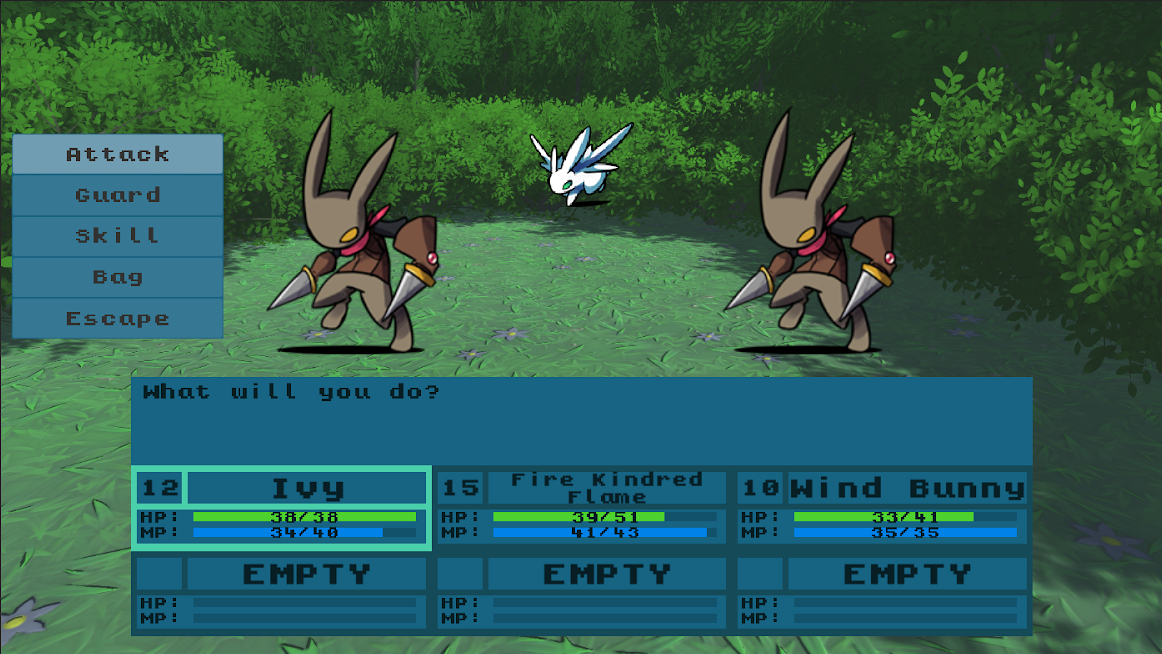
\includegraphics[width=\linewidth]{options.jpg}
     \caption{Menu de opções de ação para o demônio atualmente selecionado.}
  \end{subfigure}
  \begin{subfigure}[b]{0.5\linewidth}
    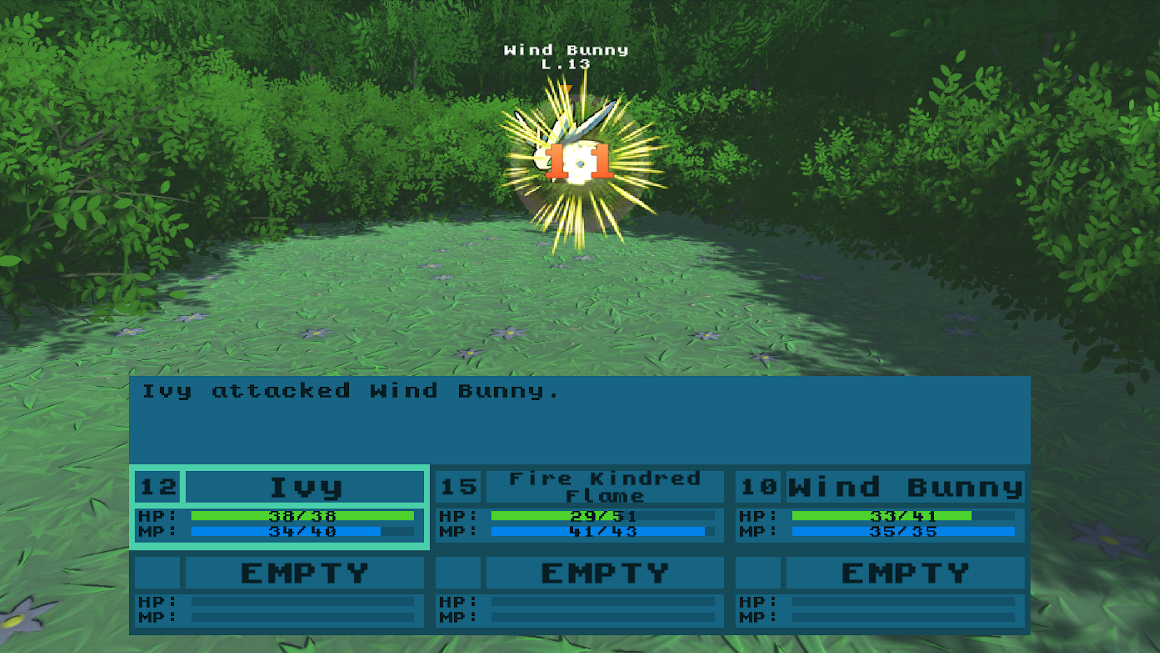
\includegraphics[width=\linewidth]{attack.jpg}
    \caption{Demônio aliado executa um ataque ao demônio inimigo.}
  \end{subfigure}
  \begin{subfigure}[b]{0.5\linewidth}
    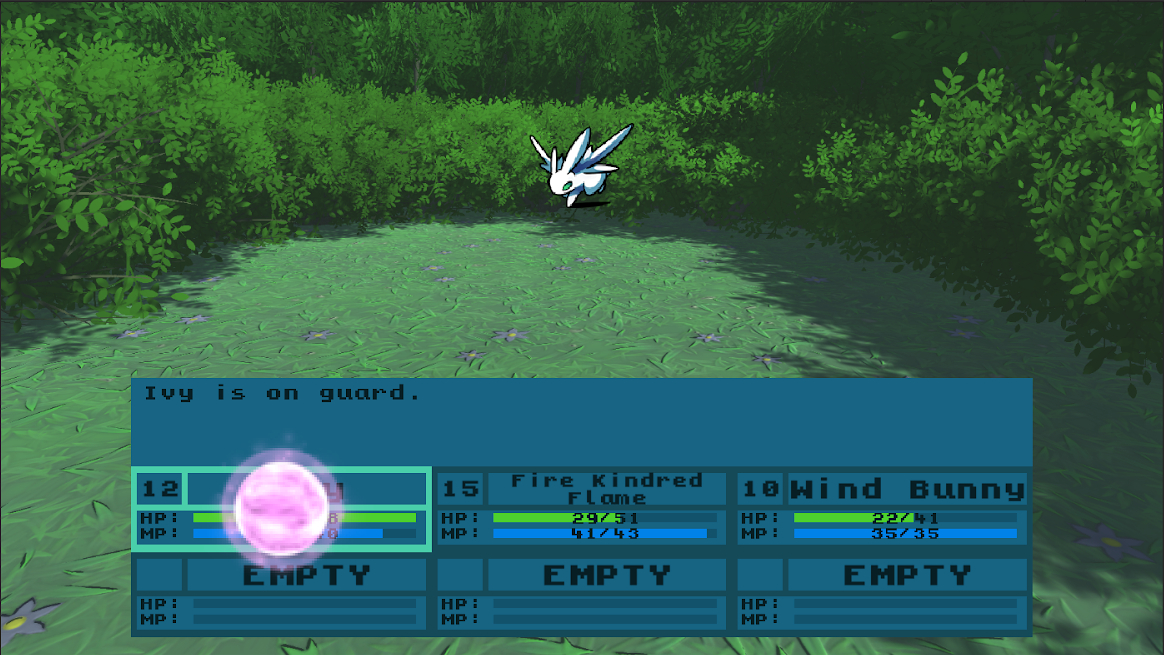
\includegraphics[width=\linewidth]{guard.jpg}
    \caption{Demônio aliado se defendendo.}
  \end{subfigure}
  \caption{Base do sistema de batalha.}
  \label{fig:battle}
\end{figure}

\subsubsection{Skills e Itens}

As skills são habilidades especiais que demônios podem utilizar durante as batalhas para causar mais dano, curar aliados, e aplicar efeitos especiais sobre aliados e inimigos ~\ref{fig:battle2}, e assim podem ser divididas em diferentes categorias: Ataque, Cura, Suporte, Efeitos Especiais, Alvos únicos, Alvos Múltiplos, Corpo a Corpo e A distância.

Skills por serem ações de batalha mais impactantes requerem que o usuário “pague” um custo dependendo do impacto da skill para utilizá-las. Skills corpo a corpo custam HP e a distância custam MP, as habilidades e personagens são balanceados de forma que os personagens que podem aprender skills a distância poderosas possuem mais MP, mas são mais frágeis, e os personagens que possuem skills corpo a corpo fortes possuem mais HP e são mais robustas.

Skills que causam dano também podem ter atributos \emph{Tipo} diferentes, sendo mais ou menos efetivas dependendo da resistência do alvo contra o \emph{Tipo} da skill.


\begin{figure}[h!]
  \centering
  \begin{subfigure}[b]{0.49\linewidth}
    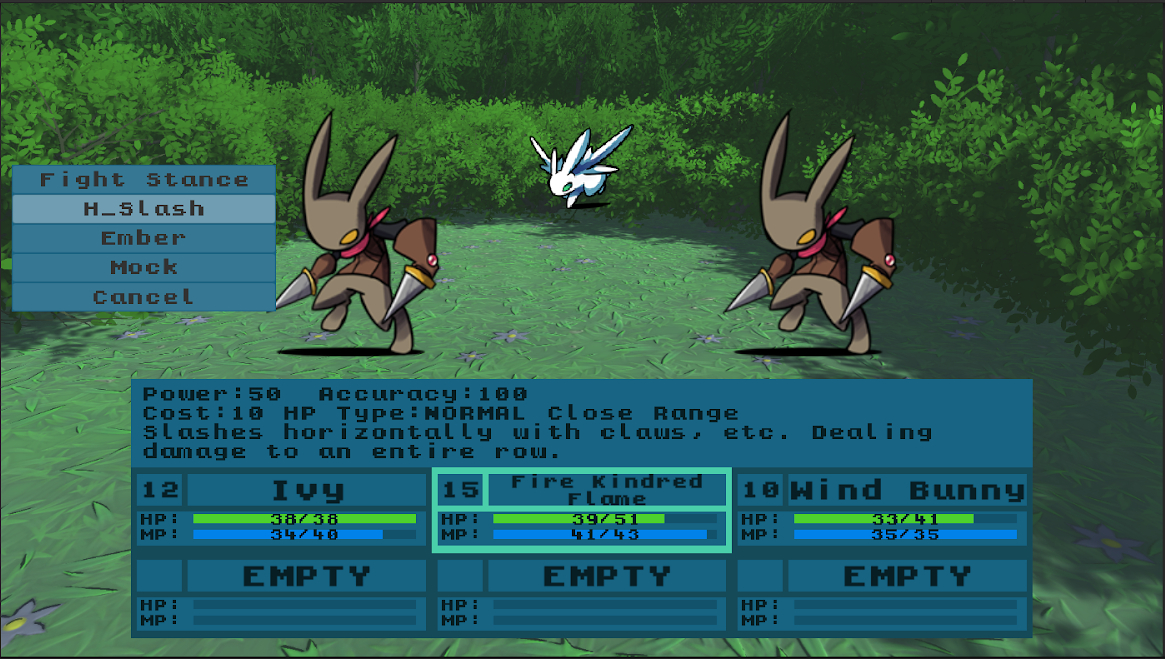
\includegraphics[width=\linewidth]{skillmenu.jpg}
     \caption{Submenu de skills do demônio selecionado.}
  \end{subfigure}
  \begin{subfigure}[b]{0.49\linewidth}
    \includegraphics[width=\linewidth]{aoe.jpg}
    \caption{Demônio utilizando uma skill que causa dano em uma linha de inimigos.}
  \end{subfigure}
  \begin{subfigure}[b]{0.49\linewidth}
    \includegraphics[width=\linewidth]{heal.jpg}
    \caption{Demônio aliado utilizando skill de cura em um companheiro.}
  \end{subfigure}
  \begin{subfigure}[b]{0.49\linewidth}
    \includegraphics[width=\linewidth]{support.jpg}
    \caption{Demônio aliado utilizando skill de suporte a aliado.}
  \end{subfigure}
  \caption{Sistema de skills em funcionamento.}
  \label{fig:battle2}
\end{figure}

Itens ~\ref{fig:itens} funcionam de maneira semelhante à skills, podendo ser utilizados por qualquer demônio aliado e a quantidade do item ao ser utilizado é reduzido por 1.

\begin{figure}[h!]
 \centering
  \includegraphics[width=0.5\linewidth]{itemmenu.jpg}
  \caption{Submenu para uso dos itens.}
  \label{fig:itens}
\end{figure}

\subsubsection{Status Effects}

\emph{Status Effects} ou "efeitos de status" são efeitos que afetam a capacidade do demônio de batalhar, podendo ser condições especiais como paralisia, ou \emph{buffs} e \emph{debuffs}.

Esses efeitos podem ser aplicados a demônios aliados e inimigos por meio de \emph{skills} e itens dando assim maior profundidade e complexidade estratégica ao construir uma equipe de demônios e ao utilizar cada demônio eficientemente em batalha. 


\subsubsection{Posição dentro da equipe}\label{info:position}

Cada grupo de demônios, sendo aliados ou inimigos, possuem uma linha frontal e uma linha posterior ~\ref{fig:battle3}. Demônios na linha frontal são mais prováveis  de serem atacados por demônios inimigos, e demônios na linha posterior causam e recebem menos dano por golpes corpo a corpo.

\begin{figure}[h!]
  \centering
  \begin{subfigure}[b]{0.5\linewidth}
    \includegraphics[width=\linewidth]{enemyformation.jpg}
     \caption{Formação de batalha dos inimigos.}
  \end{subfigure}
  \begin{subfigure}[b]{0.5\linewidth}
    \includegraphics[width=\linewidth]{partyformation.jpg}
    \caption{Formação de batalha do equipe aliada.}
  \end{subfigure}
  \caption{Posição dos aliados e inimigos em uma batalha.}
  \label{fig:battle3}
\end{figure}

\subsubsection{Captura de Demônios}

Uma das principais maneiras do jogador aumentar sua força para progredir no jogo é capturar novos demônios para utilizar em sua jornada. Todos os demônios inimigos que o jogador podem ser capturados
terminar de fazer isso aqui

\subsubsection{Progressão de personagens}\label{progression}

	A progressão de cada demônio individual do jogo é medida por meio de seu nível, que é utilizado para calcular cada um de seus \emph{stats}. Após cada batalha os demônios do jogador ganham pontos de experiencia que são responsáveis por aumentar o nível de um demônio. A quantidade de experiencia ganha é mostrada na tela de resultados ao final de cada batalha como é visto na figura ~\ref{fig:exp}.
	
\begin{figure}[h!]
 \centering
  \includegraphics[width=0.5\linewidth]{endscreen.jpg}
  \caption{A tela de final de batalha mostra a exp e itens ganhos.}
  \label{fig:exp}
\end{figure}

	Cada demônio pode aprender \emph{skills} novas ao chegar em níveis específicos assim assim aumentando o arsenal de opções que o jogador tem ao seu dispor durante as batalhas. Caso um ou mais demônios possam aprender uma \emph{skill} nova ao alcançar um nível novo, uma tela é aberta um demônio por vez para que o jogador possa escolher qual das \emph{skills} deseja deletar ~\ref{fig:learn}.
	
\begin{figure}[h!]
 \centering
  \includegraphics[width=0.5\linewidth]{learn.jpg}
  \caption{Ao aprender mais de 5 skills, o demônio deve esquecer uma.}
  \label{fig:learn}
\end{figure}

	Alguns demônios ao chegarem em certos limiares de nível podem evoluir para espécies mais poderosas de demônios, a figura ~\ref{fig:evolution} apresenta a linha evolutiva de um dos demônios que o jogador pode receber no início do jogo.
	
\begin{figure}[h!]
  \centering
  \begin{subfigure}[b]{0.2\linewidth}
    \includegraphics[width=\linewidth]{stage1.png}
     \caption{Estágio 1.}
  \end{subfigure}
  \begin{subfigure}[b]{0.3\linewidth}
    \includegraphics[width=\linewidth]{stage2.png}
    \caption{Estágio 2.}
  \end{subfigure}
  \begin{subfigure}[b]{0.45\linewidth}
    \includegraphics[width=\linewidth]{stage3.png}
    \caption{Estágio 3.}
  \end{subfigure}
  \caption{Linha evolutiva de um dos demônios do jogo.}
  \label{fig:evolution}
\end{figure}

\section{Interface}

A interação com o jogo é feita em grande parte por menus pelos quais o jogador têm várias opções de ação apresentados a ele, como exemplo na figura ~\ref{fig:menus} abaixo podemos ver o menu de ações de batalha, o menu de skills e o menu de itens, o qual é instanciado sempre vazio. Os menus estáticos têm sempre o mesmo número de opções, como é o caso dos menus de ação e o de skills, mas o menu que representa os itens por ter tamanho variável é feito como um menu que apresenta barra de rolagem.

\begin{figure}[h!]
  \centering
  \begin{subfigure}[b]{0.25\linewidth}
    \includegraphics[width=\linewidth]{menutemplate.jpg}
     \caption{Template dos menus de ação.}
  \end{subfigure}
  \begin{subfigure}[b]{0.35\linewidth}
    \includegraphics[width=\linewidth]{skilltemplate.jpg}
    \caption{Template dos menus de skills.}
  \end{subfigure}
  \begin{subfigure}[b]{0.35\linewidth}
    \includegraphics[width=\linewidth]{bagtemplate.jpg}
    \caption{Template do menu de itens.}
  \end{subfigure}
  \caption{Template dos menus utilizados durante o jogo.}
  \label{fig:menus}
\end{figure}

Para apresentar as informações essenciais para o jogador durante o jogo, foram criados diversas telas com informações de fácil acesso e entendimento ~\ref{fig:interfaces}. Durante a batalha os status de cada demônio são apresentados por meio de caixas que mostram a condição do demônio aliado, ao final de uma batalha a tela de resultados mostra ao jogador o que ele ganhou ao final da batalha, e durante o jogo o jogador tem acesso a telas de informações sobre cada demônio obtido durante o jogo.

\begin{figure}[h!]
  \centering
  \begin{subfigure}[b]{0.55\linewidth}
    \includegraphics[width=\linewidth]{resultstemplate.jpg}
     \caption{Template da tela de resultados.}
  \end{subfigure}
  \begin{subfigure}[b]{0.55\linewidth}
    \includegraphics[width=\linewidth]{statstemplate.jpg}
    \caption{Template da tela de stats.}
  \end{subfigure}
  \begin{subfigure}[b]{0.3\linewidth}
    \includegraphics[width=\linewidth]{hudtemplate.jpg}
    \caption{Template da HUD.}
  \end{subfigure}
  \caption{Template de diversas interfaces criadas para o jogo.}
  \label{fig:interfaces}
\end{figure}

\section{Cidades}\label{cidades}

As cidades dentro do jogo nasceram da necessidade de se existir um local considerado seguro onde o jogador poderia fazer ações como curar seus demônios, trocar demônios do grupo com demônios salvos no demonomicon, e para se ter um elemento narrativo que sirva de objetivo e propósito para o jogador.
	
	Um dos NPCs criados para habitar a cidade é o Mestre da Guilda, o jogador o encontra ao entrar na Guilda. Ao encontrar com o Mestre da Guilda o jogador recebe seu primeiro demônio, alguns itens para iniciar a aventura e uma missão em troca do demônio inicial.

	O segundo NPC implementado é a Demonóloga, que dá ao jogador um meio de curar seus demônios, invocar demônios do demonomicon e selar demônios do grupo de volta para o demonomicon.

\chapter{Desenvolvimento}

Neste capítulo será detalhado o processo de desenvolvimento do jogo, que consiste na implementação das decisões de design feitas durante a etapa de design inicial e durante a revisão de \emph{feedback} recebidos durante a etapa de teste.

\section{Ferramentas}

As ferramentas mais utilizadas durante o projeto foi o motor de jogos Unity ~\ref{fig:editor}, e o editor de imagens GIMP (GNU Image Manipulation Program) ~\ref{fig:gimp} o qual foi utilizado para a criação e edição de \emph{assets} gráficos por ser uma poderosa ferramenta para edição de imagens, open source, gratuita e fácil de utilizar.

\begin{figure}[h!]
 \centering
  \includegraphics[width=0.70\linewidth]{unityeditor.jpg}
  \caption{Editor do motor de jogos Unity.}
  \label{fig:editor}
\end{figure}

\begin{figure}[h!]
 \centering
  \includegraphics[width=0.70\linewidth]{gimp.jpg}
  \caption{Workspace do GIMP.}
  \label{fig:gimp}
\end{figure}

Outras ferramentas utilizadas para a criação do jogo foram: Visual Studio Code para escrita de código;
Github Desktop para o versionamento do projeto; Google Docs, Google Meet, e e-mail para a
comunicação com o orientador e manter o controle de horas trabalhadas e a plataforma Itch.io em conjunto com o Google Forms e Discord para os testes com jogadores.

\section{Assets}

Para concentrar o esforço de criação do jogo na implementação de sistemas e lógica de jogo a maior parte dos assets gráficos e todos os assets sonoros são \emph{Royalty-free} obtidos de diversas fontes encontradas online, sendo a maioria encontrada no Itch.io. %lembrar de como referenciar os assets utilizados em referencias


\section{Arquitetura das Mecânicas de Exploração}


\subsection{Representação do jogador}

O jogador, como é representado durante a exploração do labirinto, é um objeto 3D ~\ref{fig:playerobject} com duas câmeras acopladas, a primeira é a câmera principal que dá o jogo a visão em primeira pessoa, já a segunda se encontra bem acima do jogador, a qual gera a imagem reproduzida pelo mini mapa do jogo.
 

\begin{figure}[h!]
 \centering
  \includegraphics[width=0.65\linewidth]{playerobject.jpg}
  \caption{O objeto \emph{OverworldPlayer} visto pelo editor Unity.}
  \label{fig:playerobject}
\end{figure}

Atrelado à caixa de colisão do jogador há rotinas que definem como o jogador consegue interagir com o ambiente do labirinto, como interação com os itens e objetos interativos, e zonas especiais que indicam quando e como encontros aleatórios e eventos especiais, tais como tutoriais, ocorrem durante a exploração do labirinto.

\subsection{Random Encounters}

Os diferentes métodos de realizar encontros aleatórios estudados foram os encontrados nos jogos da primeira geração de \emph{Pokémon} e em \emph{Etrian Odyssey V}.

Em \emph{Etrian Odyssey V}, ao entrar no labirinto ou após cada batalha, um número aleatório de 64 a 256 é setado como limite de um contador, e cada espaço do labirinto em que o jogador pode dar um passo têm a ele associado um valor de 0 a 20, o qual é adicionado ao contador cada vez que o jogador entra em um desses espaços. Quando o contador ultrapassa o limite definido uma encontro aleatório é iniciado de acordo com uma tabela que indica quais são os possíveis encontros que o jogador pode batalhar em cada espaço. Este método garante que o jogador possa dar um número minimo de passos antes que encontre outra batalha, e permite que os designers façam ajustes finos a taxa de encontros para que a experiencia do jogador não se torne frustrante durante o jogo. A desvantagem deste método é grande quantidade de recursos que se deve ser alocada a implementação da mecânica, dado que cada passo do labirinto deve ser ajustado e reajustado a cada modificação do design do labirinto.

Em \emph{Pokémon}, a cada passo que o jogador executa dentro de áreas onde pode encontrar pokémons selvagens é gerado um valor aleatório entre 0 e 255, este valor então é comparado com a taxa de encontro da àrea em que se encontra, caso o valor gerado seja maior que a taxa de encontro o jogo inicia uma batalha. A espécie e nível do pokémon selvagem gerado para esse encontro é decidido a partir de uma tabela de encontros. A vantagem deste método é de ser muito simples e facil de implementar no jogo, a desvantagem é que prejudica a exploração em áreas onde não se pode desviar de zonas em que encontros aleatórios ocorrem ou em áreas com taxa de encontro muito altas.

Para o jogo desenvolvido para este trabalho, se optou por uma estratégia semelhante à utilizada em \emph{Etria Odyssey V} porém simplificada para ficar coerente com o escopo do trabalho. O labirinto foi dividido em diversas zonas com diferentes valores Xi, e tabelas de encontros associados a eles, e a cada passo que o jogador executa dentro dessas zonas se adiciona o valor Xi a um contador. Uma batalha é iniciada quando o contador Xi ultrapassa um certo valor Y definido como limite, e o grupo de demônios que é encontrado é decidido aleatoriamente a partir da tabela de encontros associada a área em que o jogador se encontra.
\pagebreak
\lstinputlisting[language=json, firstline=1, lastline=36, caption = {Trecho do arquivo JSON que contêm os encontros por zoneID}, label={lst:encounterTable}]{EncounterTable.json}

No trecho de código apresentado em \ref{lst:encounterTable} podemos ver em detalhes como o jogo gera o grupo de inimigos que o jogador encontra em cada encontro aleatório, de acordo com a \emph{zoneID} de cada área explorável do mapa, o algoritmo escolhe aleatoriamente dentro da \emph{encounterList} um grupo de inimigos de nível entre \emph{min\textunderscore level} e \emph{max\textunderscore level} e com a formação \emph{enemy\textunderscore formation} contra qual o jogador deve batalhar.

\subsection{Labirinto}

	Todo labirinto antes de ser implementado dentro do jogo é criado utilizando um software gratuito chamado Dungeon Map Doodler, que permite a criação de mapas de RPGs de tabuleiro de maneira semelhante a lápis e papel. O uso deste método tornou mais rápido e eficaz o processo de criação de novos labirintos para o jogo.Na figura ~\ref{fig:dungeonLayout} temos um exemplo de um dos \emph{layout} criados para um labirinto do jogo.
	
\begin{figure}[h!]
  \centering
  \begin{subfigure}[b]{0.45\linewidth}
    \includegraphics[width=\linewidth]{encounterZones.png}
     \caption{Layout do labirinto com suas diferentes zonas.}
  \end{subfigure}
  \begin{subfigure}[b]{0.45\linewidth}
    \includegraphics[width=\linewidth]{dungeonItens.png}
    \caption{Layout do labirinto com a posição de todos itens.}
  \end{subfigure}
  \caption{Layout de um labirinto criado com Dungeon Map Doodler.}
  \label{fig:dungeonLayout}
\end{figure}

	A estrutura básica dos labirintos se resume a paredes que são visíveis apenas pela câmera do minimapa, caixas de colisão que definem as diferentes zonas do labirinto e a objetos interativos espalhados com os quais o jogador pode interagir, como está ilustrado na figura ~\ref{fig:basicLab}.

\begin{figure}[h!]
  \centering
  \begin{subfigure}[b]{0.75\linewidth}
    \includegraphics[width=\linewidth]{basicLab.png}
     \caption{Visão superior da estrutura básica de um labirinto.}
  \end{subfigure}
  \begin{subfigure}[b]{0.75\linewidth}
    \includegraphics[width=\linewidth]{basicLab2.png}
    \caption{Visão ortogonal da estrutura básica de um labirinto.}
  \end{subfigure}
  \caption{Estrutura básica de uma labirinto de duas perspectivas diferentes.}
  \label{fig:basicLab}
\end{figure}

Para dar vida e tornar os labirintos visualmente interessantes foi utilizado o sistema de terrenos disponível pelo motor de jogos Unity em conjunto a \emph{assets} gratuitos para representação de árvores, arbustos, chão e água encontrados no Itch.io e na loja de \emph{assets} do Unity. O terreno foi desenhado estrategicamente para dar a ilusão ao jogador de que ele está colidindo com o terreno, quando na realidade todas colisões são com as paredes invisíveis. O resultado da adição do terreno pode ser observado na figura ~\ref{fig:terrain}

\begin{figure}[h!]
 \centering
  \includegraphics[width=0.75\linewidth]{prettyLab.png}
  \caption{Visão ortogonal de um labirinto com terreno adicionado.}
  \label{fig:terrain}
\end{figure}

\subsection{Overworld Menu System}

	Durante a exploração dos labirintos, as ações que o jogador pode fazer utilizando o menu ~\ref{owmenu} estão implementadas no arquivo OW\_MenuSystem.cs, que por meio de uma máquina de estados foram criadas ações bem definidas como abrir menus, utilizar itens e abrir caixas de dialogo uteis para o progresso do jogador.

\section{Arquitetura das Mecânicas de Batalha}

\subsection{Arena de Batalha}

	A cena de batalha é composta basicamente de partes diferentes, o \emph{background} tridimensional que representa a arena de batalha, o grupo dos inimigos, e o grupo do jogador.
	
	O \emph{Background} é uma arena construída com os mesmos \emph{assets} tridimensionais utilizadas na construção do labirinto e uma câmera auxiliar renderiza a imagem da arena sobre um plano bidimensional atrás dos objetos da cena que são capturados pela câmera principal, como ilustra a figura ~\ref{fig:background}.
	
\begin{figure}[h!]
  \centering
  \begin{subfigure}[b]{0.75\linewidth}
    \includegraphics[width=\linewidth]{arena.png}
     \caption{Arena construida com \emph{assets} tridimensionais.}
  \end{subfigure}
  \begin{subfigure}[b]{0.75\linewidth}
    \includegraphics[width=\linewidth]{background.png}
    \caption{Background projetado sobre um plano bidimensional.}
  \end{subfigure}
  \caption{Visão da cena de Batalha como é vista pelo editor.}
  \label{fig:background}
\end{figure}


\subsection{Demônios}

	Demônios são os objetos dentro do jogo com os quais o jogador deve utilizar para derrotar outros demônios encontrados dentro dos labirintos, cada demônio encontrado dentro do jogo é membro de uma espécie, que define seu \emph{sprite} (imagem bidimensional) que o representa, seus \emph{stats} e quais \emph{skills} pode aprender.
	
	As definições de \emph{stats} base de cada demônio estão escritas no arquivo BaseStats.cs ~\ref{lst:basestats}, e os golpes que cada demônio pode aprender estão definidos no arquivo MovePool.cs ~\ref{lst:movepool}.
	

	
\lstset{style=sharpc, caption={Exemplo da inserção de uma espécie de demônio dentro do jogo}, label={lst:basestats}}
\begin{lstlisting}
new DemonStats (/*name*/ "Carnidos",
                             /*HP*/    60,
                             /*MP*/    70, 
                             /*ATK*/   62, 
                             /*DEF*/   63, 
                             /*SPATK*/ 80, 
                             /*SPDEF*/ 80, 
                             /*SPEED*/ 60,
                             /*TYPE*/  TYPE.GRASS,
                             /*CATCH*/ 45,
                             /*EXP*/   141,
                             /*GROWTH*/GROWTH_RATE.MEDIUM_SLOW,
                             /*EVOID*/ "Carnivotres",
                             /*EVOLVL*/30)
\end{lstlisting}

\lstset{style=sharpc, caption={Exemplo da definição de golpes aprendíveis por nível de um demônio}, label={lst:movepool}}
\begin{lstlisting}
new Demon_MovePool("Carnidos", 
            new List<LevelUp_Move>(new[] {
                new LevelUp_Move(/*Level*/1, /*skillID*/5),
                new LevelUp_Move(/*Level*/3, /*skillID*/1),
                new LevelUp_Move(/*Level*/5, /*skillID*/18),
                new LevelUp_Move(/*Level*/6, /*skillID*/6),
                new LevelUp_Move(/*Level*/9, /*skillID*/39),
                new LevelUp_Move(/*Level*/13, /*skillID*/4),
                new LevelUp_Move(/*Level*/16, /*skillID*/14),
                new LevelUp_Move(/*Level*/18, /*skillID*/26)
                }))
\end{lstlisting}

\subsection{Calculo de Stats}\label{chap:Stats}

	O método de calculo dos \emph{stats} de cada demônio foi baseado no método utilizado nos jogos da franquia Pokémon, onde os \emph{stats} são calculados a partir de fórmulas que levam em conta os \emph{stats} base da espécie do pokémon, do nível, e de alguns atributos individuais. Este método foi escolhido pois outros métodos estudados, que envolviam a definição manual de como os \emph{stats} de cada personagem do jogo crescem por nível, ou o uso de "lançamento de dados" para definir o crescimento de cada personagem ao ganhar um nível, foram descartados por serem ineficientes para a grande quantidade de demônios presentes no jogo ou por serem mais difíceis de balancear por dependerem de números gerados aleatoriamente.
	
	As fórmulas ~\ref{eqn:HP}, ~\ref{eqn:MP} e ~\ref{eqn:Other} foram  utilizadas para o cálculo dos \emph{stats} de cada demônio a partir dos \emph{stats} base da espécie, nível Level do demônio, nível máximo MaxLevel e duas constantes X e Y definidas por meio de teste.
	
\begin{equation}
\label{eqn:HP}
HP = X*baseHP * Level/MaxLevel + Level + 2*Y
\end{equation}

\begin{equation}
\label{eqn:MP}
MP = X*baseMP * Level/MaxLevel + Level + 2*Y
\end{equation}

\begin{equation}
\label{eqn:Other}
OutrosStats = X*baseSTAT * Level/MaxLevel + Y
\end{equation}

	A fórmula ~\ref{eqn:TotalExp} define quantos de pontos de experiencia totais um demônio deve ter para alcançar um nível Level dado um fator de crescimento G dependente da taxa de crescimento da espécie e um valor constante E de experiencia base.
	
\begin{equation}
\label{eqn:TotalExp}
TotalEXP = E * Level^G
\end{equation}

	A fórmula ~\ref{eqn:Exp} define quantos pontos de experiencia cada demônio inimigo fornece ao ser derrotado com base na EXP base da espécie, do seu nível Level e constante Z determinada por meio de testes.
	
\begin{equation}
\label{eqn:Exp}
YieldEXP = EXP * Level/Z
\end{equation}


\subsection{Skills e Itens}

	As \emph{Skills} foram implementadas como um classe no script SkillData.cs, e todas as \emph{Skills} devem estão salvas em uma lista \emph{SkillList} com informações necessária para o uso de cada \emph{skill}: nome, tipo elemental, tipo de alvo, prioridade, poder, precisão, custo, efeito especial, se é especial, se é de longa distancia, ID (número de identificação),  efeito visual, cor do efeito visual, descrição e se é utilizável durante a exploração do labirinto. Um exemplo de como uma \emph{skill} é adicionada ao jogo pode ser vista no trecho de código retirado de SkillData.cs ~\ref{lst:skilldata}.

\lstset{style=sharpc, caption={Exemplo de como uma \emph{skill} é adicionada ao jogo}, label={lst:skilldata}}
\begin{lstlisting}
new SkillData (/*name*/        "Absorb", 
               /*type*/         BaseStats.TYPE.GRASS, 
               /*target_type*/  TARGET_TYPE.SINGLE, 
               /*priority*/     PRIORITY.NORMAL, 
               /*power*/        30, 
               /*accuracy*/     100, 
               /*cost*/         6,
               /*effect*/       new EFFECT[] {EFFECT.LIFESTEAL}, 
               /*isSpecial*/    true, 
               /*isRanged*/     true,
               /*ID*/           6,
               /*VFX*/          "Absorb",
               /*VFX_COLOR*/    new Color(0, 1, 0.93f, 1),
               /*DESC*/         "An attack that absorbs half the damage inflicted.",
               /*OWuse*/        false),
\end{lstlisting}

	Os itens foram implementados a partir da implementação das \emph{skills} em uma classe \emph{Item} no arquivo ItemData.cs, e por isso são adicionadas ao jogo praticamente da mesma maneira que as \emph{skills}, porém em uma lista \emph{ItemList}. Um exemplo de como um item é adicionado ao jogo pode ser vista no trecho de código retirado de ItemData.cs ~\ref{lst:itemdata}.
	
\lstset{style=sharpc, caption={Exemplo de como um item é adicionado ao jogo}, label={lst:itemdata}}
\begin{lstlisting}
new ItemData (/*name*/        "H_UltraPotion", 
              /*type*/         BaseStats.TYPE.NORMAL, 
              /*target_type*/  Skill.TARGET_TYPE.ALLY_ROW, 
              /*priority*/     PRIORITY.NORMAL, 
              /*power*/        -40, 
              /*accuracy*/     100, 
              /*cost*/         0,
              /*status_effect*/new Skill.EFFECT[] {Skill.EFFECT.NULL}, 
              /*isSpecial*/    true, 
              /*isRanged*/     true,
              /*ID*/           5,
              /*VFX*/          "Heal",
              /*VFX_COLOR*/    new Color(0.6f, 1.0f, 0.92f, 1.0f),
              /*DESC*/         "Medicine that recovers a great amount HP of an entire row.",
              /*OWuse*/        true)
\end{lstlisting}

	As animações que tocam quando se utiliza um item ou uma skill são determinadas pelo campo VFX que define qual animação deve ser mostrada ao jogador, e devido a quantidade limitada de animações disponíveis gratuitamente, o campo VFX\_COLOR define a cor da animação, criando a possibilidade de se utilizar a mesma animação para diferentes efeitos.

	O parâmetro OWuse indica quais \emph{skills} ou itens podem ser utilizados durante a exploração do labirinto, já que alguns itens e \emph{skills} possuem utilidade apenas em batalha.

\subsection{Calculos de Dano}

	Em jogos RPG há 3 maneiras diferentes de se calcular dano, primeiro de forma que o dano é resultado da força do ataque subtraido pela defesa do alvo ~\ref{eqn:F1} como é visto em \emph{Etrian Odyssey}; a segunda forma é o dano mitigado pela defesa ser uma porcentagem do valor total do ataque ~\ref{eqn:F2} como é feito em jogos MOBAs (\emph{Multiplayer Online Battle Arena}), como por exemplo em \emph{League Of Legends}; e por ultimo o dano é resultado da razão entre o poder de ataque do atacante e o poder de defesa do defensor ~\ref{eqn:F3} como é feito por exemplo em \emph{Pokémon}.
	
\begin{equation}
\label{eqn:F1}
DMG = ATK - DEF
\end{equation}

\begin{equation}
\label{eqn:F2}
DMG = ATK * (1 - DEF/MAXDEF)
\end{equation}

\begin{equation}
\label{eqn:F3}
DMG = ATK / DEF
\end{equation}

	Como o ataque, defesa e quantidade de vida dos demônios são calculados a partir de valores básicos são proporcionais ao nível do demônio, como visto no capítulo ~\ref{chap:Stats}, foi decidido que a implementação do calculo de dano seria baseado na equação ~\ref{eqn:F3} resultando na formula \ref{eqn:damage}.

\begin{equation}
\label{eqn:damage}
(X*\frac{ATKLVL}{Y} + Z) * \frac{SPOWER}{BPOWER} * \frac{ATK*ATKMOD}{DEF*DEFMOD} * DEFLANE * ATKLANE * RES * COND
\end{equation}

	Na equação ~\ref{eqn:damage} temos que o valores X, Y e Z são valores constantes decididos por experimentação, SPOWER é o poder do ataque, BPOWER é o valor base da ação \emph{ATTACK} ~\ref{chap:BattleOptions}, ATK é o \emph{ATK} ou \emph{SP.ATK} ~\ref{info:stats} do demônio atacante dependendo se o ataque é de curta ou longa distancia respectivamente, DEF é o \emph{DEF} ou \emph{SP.DEF} ~\ref{info:stats} do demônio defensor dependendo se o ataque é de curta ou longa distancia respectivamente, ATKMOD e DEFMOD são dependente dos modificadores de ataque e defesa dos demônios atacante e defensor respectivamente, DEFLANE e ATKLANE são modificadores referentes a posição das unidades defensoras e atacantes para casos em que o ataque é corpo a corpo de acordo com a decisão de design vista em ~\ref{info:position}, RES é o modificador baseado na resistência do defensor contra o tipo do ataque de acordo com a tabela ~\ref{resistance}, e por fim COND é um valor referente a condições especiais que estejam afetando o demônio atacante.
	
	A função para o calculo de cura é semelhante, mas mais simples, à função de dano, pois não leva em consideração a defesa do alvo e pode ser vista na equação ~\ref{eqn:heal}.

\begin{equation}
\label{eqn:heal}
(X*\frac{ATKLVL}{Y} + Z) * \frac{SPOWER}{BPOWER} 
\end{equation}


\subsection{Precisão e Esquiva}

A precisão de golpes é calculada pela formula ~\ref{eqn:accuracy} onde ACC é a precisão da habilidade ACCMOD é o modificador de precisão resultante de efeitos especiais aplicados sobre o demônio que executa a ação, e EVA é o modificador de evasão resultante de efeitos especiais aplicados sobre o demônio alvo.

\begin{equation}
\label{eqn:accuracy}
TOTALACC = ACC * ACCMOD / EVA
\end{equation}

	A precisão resultante então é comparada com um número gerado aleatoriamente de 1 a 100, caso a precisão resultante seja o maior, o golpe acerta o alvo, caso negativo, o golpe não acerta o alvo e nada acontece.

\subsection{Buffs e Debuffs}

	Quando um \emph{stat} de um demônio é utilizado para algum calculo em batalha, um número de modificadores podem ser aplicados durante os cálculos. Durante a batalha, os \emph{stats} efetivos de um demônio pode ser aumentado ou diminuido por algumas \emph{skills}, que são chamadas de \emph{Buffs} e \emph{Debuffs} respectivamente.
	
	Os modificadores operam em uma escala deslizante de estágios. quando um dado \emph{stat} é elevado ou diminuído, o seu estágio atual é aumentado ou diminuído pela quantidade ditada pela \emph{skill}, até um máximo de +6 e um mínimo de -6. Um dado estágio corresponde a um dado multiplicador que irá modificar o \emph{stat} quando ele é utilizado para calculos de batalha. Os multiplicadores exatos para cada estagio estão detalhados na tabela ~\ref{tab:stages}.
	
\begin{table}[!htp]\centering
\caption{Stats Modifiers Table}\label{tab:stages}
\scriptsize
\begin{tabular}{lrrrrrrrrrrrrrr}\toprule
Stage &-6 &-5 &-4 &-3 &-2 &-1 &0 &1 &2 &3 &4 &5 &6 \\\cmidrule{1-14}
Modifier &2/8 &2/7 &2/6 &2/5 &2/4 &2/3 &2/2 &3/2 &4/2 &5/2 &6/2 &7/2 &8/2 \\\midrule
\bottomrule
\end{tabular}
\end{table}

\subsection{Condições Especiais}\label{conditions}

	Assim como \emph{Buffs} e \emph{Debuffs} condições especiais podem ser infligidos a demônios por meio de \emph{skills}, essas condições especiais afetam a capacidade do demônio afetado de batalhar eficientemente. Atualmente no protótipo estão implementados 5 diferentes condições especiais sendo elas:

\begin{itemize}
\item Poison
	\begin{itemize}
	\item A cada turno o demônio envenenado perde 1/8 da vida.
	\item No labirinto a cada 4 passos dado faz o demônio envenenado perder 1/16 de vida arredondado para baixo (mínimo de 1 por passo).
	\item Pode ser curada por item ou \emph{skill}.
	\item Demônios do tipo \emph{POISON} não podem ser envenenadas.
	\end{itemize}
\item Burn
	\begin{itemize}
	\item A cada turno o demônio queimado perde 1/8 da vida.
	\item O demônio queimado causa 50\% a menos de dano com golpes corpo a corpo.
	\item Pode ser curada por item ou \emph{skill}.
	\item Unidades do tipo \emph{FIRE} não podem ser queimadas.
	\end{itemize}
\item Freeze
	\begin{itemize}
	\item O demônio congelado não consegue agir.
	\item Todo turno o demônio congelado têm 20\% de chance de descongelar e pode atacar no mesmo turno que descongelar
	\item Podem ser curada por item ou \emph{skill}.
	\item O demônio é descongelado ao final da batalha.
	\item Demônios do tipo \emph{ICE} são imunes a congelamento.
	\end{itemize}
\item Paralysis
	\begin{itemize}
	\item O demônio paralisado tem 25\% de chance de perder a vez durante seu turno.
	\item A velocidade do demônio paralisado é diminuída pela metade. 
	\end{itemize}
\item Rage
	\begin{itemize}
	\item O demônio fica incapacitado de fazer qualquer ação além de \emph{ATTACK}.
	\item O demônio causa 25\% a mais de dano corpo a corpo.
	\item Podem ser curada por item ou \emph{skill}.
	\item O demônio é curado ao final da batalha.
	\end{itemize}
\end{itemize}

	Adicionalmente, existem diferentes chances de se aplicar condições especiais podendo ser uma chance baixa, uma chance alta ou em alguns poucos casos, sempre aplicam.

\subsection{Captura de demônios}
	
	A ação de capturar demônios foi implementada como um efeito especial de alguns itens criados especificamente para possibilitar que jogadores obtenham novos demônios para seu grupo. Para verificar se a ação de captura foi concluída com sucesso, um número X é calculado a partir da equação ~\ref{eqn:capture} onde maxHP é a vida máxima do demônio alvo, currentHP é a vida atual do demônio alvo, catch\_rate é um valor associado a especie do demônio alvo que define o quão fácil ele é capturado, sealBonus é um bônus associado ao item utilizado, e A é um valor definido de acordo com o game design, sendo que a chance de captura de um demônio com vida atual igual a máxima é 1/A da chance de quando o demônio está com apenas 1 HP restante.

\begin{equation}
\label{eqn:capture}
X = \frac{A * maxHP - (A-1)*currentHP}{A*maxHP}*catch\_rate*sealBonus
\end{equation}

	Caso o jogador esteja com o grupo cheio, as informações do demônio capturado são salvas dentro de um objeto chamado \emph{Demonomicon} e o jogador pode trocar os demônios que possui dentro do grupo com os salvos no \emph{Demonomicon} por meio da NPC Demonóloga ~\ref{cidades}.
	
\subsection{Sistema de Batalhas}

	As batalhas são gerenciadas pelo sistema de batalha implementado no arquivo Battle\_System.cs que por meio de uma máquina de estados divide cada turno de uma batalha em 6 estados diferentes: START; MOVESELECTIONTURN; TARGETSELECTIONTURN; BATTLETURN; WON; LOST;
	
	Durante o estado START são inicializados todos os parâmetros utilizados durante a batalha e a função SetupBattle() é chamada onde os demônios aliados e inimigos são instanciados na \emph{scene}.

	Ao iniciar a fase de escolha de ações, as ações dos inimigos são escolhidas por meio de uma algoritmo e então o sistema alterna entre os estados MOVESELECTIONTURN e TARGETSELECTIONTURN para o jogador conseguir registar as ações de todos os demônios em seu grupo.

	Após o jogador selecionar todas as ações de seus demônios, o sistema de batalha entra no  estado BATTLETURN, onde todas as ações de batalha são executadas.
	
	A ordem em que as ações são executadas dependem primeiro da prioridade da ação e em segundo da velocidade do demônio, por exemplo, se um demônio utiliza \emph{GUARD}, uma ação de prioridade alta, contra um demônio que utiliza \emph{ATTACK}, a ação \emph{GUARD} vai ser sempre executada primeiro independente da velocidade de ambos os demônios. Em outro exemplo um demônio com \emph{SPEED} 10 e outro demônio com \emph{SPEED} 11 executam ações de mesma prioridade, o demônio com \emph{SPEED} 11 sempre irá agir primeiro.

	Depois de cada ação que pode encerrar uma batalha, como por exemplo a captura ou morte de um demônio, o sistema de batalha checa condições para o fim de uma batalha, caso todos os demônios aliados sejam derrotados, o estado muda para LOST indicando que o jogador foi derrotado e retornado o jogador para a cidade, caso todos os demônios inimigos sejam derrotados, o estado muda para WIN e o sistema calcula as recompensas recebidas por vencer a batalha e inicia o processo de retornar o jogador ao labirinto.

\section{Game Manager}

	O Game Manager é um dos dois únicos objetos que não são destruídos ao se trocar de \emph{scene} dentro do jogos, sendo o outro o AudioManager, que é instanciado na primeira \emph{scene} aberta no jogo e só é destruído ao se fechar o jogo. Este comportamento é necessário pois dentro do Game Manager são salvas informações necessárias para o funcionamento do jogo como um todo, e serve como uma ponte entre as diversas \emph{scenes} que compõem o jogo.
	
	Dentro do Game Manager é salvo informações de progresso do jogador como a posição do jogador dentro do labirinto, em qual labirinto o jogador se encontra, os demônios presentes no grupo do jogador, os demônios salvos no \emph{demonomicon} e os itens que possui.
	
	Além das informações do jogador listas mantém registro dos eventos que devem acontecer dentro do jogo e quais ja aconteceram e não devem acontecer novamente, como tutoriais já vistos, quais atalhos foram desbloqueados, quais itens ja foram recolhidos do labirinto, e quais missões já foram concluídas.
	
	O Game Manager também é responsável por manter gerenciar o estado atual do jogo, e quais \emph{scenes} devem ser abertas em cada etapa do jogo. A implementação completa do Game Manager pode ser encontrado no script \emph{GameManager.cs}.
	
\section{Teste com jogadores reais}

	Depois de implementado as mecânicas básicas de exploração de labirintos, foi executado um teste com jogadores reais para avaliar o protótipo e com base no \emph{feedback} recebido implementar mudanças e novas mecânicas para melhorar a experiencia do jogador e o jogo como um todo.
	
	O participantes escolhidos para o testar a primeira iteração do protótipo foram pessoas próximas que pudessem testar o jogo pessoalmente ou com comunicação pelo Discord, pois neste estágio não estavam implementados nenhum tutorial ou ferramentas que ensinassem ao jogador o funcionamento básico de combate e exploração do jogo, necessitando assim da assistência do desenvolvedor para um teste bem sucedido.

	Para auxiliar na coleta de \emph{feedback} foi utilizado um Google Forms que todos os jogadores responderam após testarem o jogo. O resultado das perguntas de múltiplas escolhas pode ser vista na figura ~\ref{fig:feedback}.
\pagebreak

\begin{figure}[h!]
  \centering
  \begin{subfigure}[b]{0.49\linewidth}
    \includegraphics[width=\linewidth]{forms1.png}
  \end{subfigure}
  \begin{subfigure}[b]{0.49\linewidth}
    \includegraphics[width=\linewidth]{forms2.png}
  \end{subfigure}
  \begin{subfigure}[b]{0.49\linewidth}
    \includegraphics[width=\linewidth]{forms3.png}
  \end{subfigure}
  \begin{subfigure}[b]{0.49\linewidth}
    \includegraphics[width=\linewidth]{forms4.png}
  \end{subfigure}
  \begin{subfigure}[b]{0.49\linewidth}
    \includegraphics[width=\linewidth]{forms5.png}
  \end{subfigure}
  \begin{subfigure}[b]{0.49\linewidth}
    \includegraphics[width=\linewidth]{forms6.png}
  \end{subfigure}
  \begin{subfigure}[b]{0.49\linewidth}
    \includegraphics[width=\linewidth]{forms7.png}
  \end{subfigure}
  \begin{subfigure}[b]{0.49\linewidth}
    \includegraphics[width=\linewidth]{forms8.png}
  \end{subfigure}
  \begin{subfigure}[b]{0.49\linewidth}
    \includegraphics[width=\linewidth]{forms9.png}
  \end{subfigure}
  \begin{subfigure}[b]{0.49\linewidth}
    \includegraphics[width=\linewidth]{forms10.png}
  \end{subfigure}
  \caption{Respostas das perguntas de múltiplas escolhas.}
  \label{fig:feedback}
\end{figure}

	Outras perguntas feitas no Forms foram: Qual foi o momento ou aspecto mais frustrante durante o jogo?; Qual foi momento ou aspecto que mais te agradou durante o jogo?; Teve alguma coisa que você queria fazer mas não pôde?; Se pudesse, o que você gostaria de mudar, adicionar, ou remover da experiência?; Como você descreveria o jogo para uma familiar ou amigo?.
	
	A análise dos \emph{feedbacks} levou as seguintes melhorias que deveriam ser implementas em uma segunda iteração:

\begin{itemize}
\item Precisa aumentar a quantidade de XP que se obtém por batalha, ou melhorar o balanceamento de inimigos.
\item Habilidade de buff e debuff precisam ser mais fortes para incentivar uso pelos jogadores.
\item Aumentar a variedade de habilidades e efeitos.
\item Ensinar melhor o jogador a jogar.
\item Não rotacionar o mapa para causar menos desorientação ao jogador.
\item Melhor a claridade de quando golpes são super efetivos, são pouco efetivos e quando golpes erram o alvo.
\item Quando o alvo for um monstro que já está morto, focar o próximo alvo.
\item Criar uma tela de resultado de batalha para maior visibilidade.
\end{itemize}

\section{Melhorias feitas com base no \emph{feedback} dos jogadores}

	Com base nos testes com jogadores, uma segunda iteração do protótipo foi implementada, nesta segunda iteração foram feitos ajustes pequenos como retirar a rotação do minimapa, ajustes na quantidade de experiencia que os demônios aliados ganham em batalha, mudanças visuais para indicar quando golpes causam dano super-efetivo ou pouco efetivos, adição de elementos interativos no labirinto ~\ref{chap:interactables}, criação de uma tela de resultados exibida ao final de batalhas ~\ref{progression}, redirecionamento de ações que têm como alvo demônios mortos, e melhorias feitas aos tutoriais. Também foi necessário ajustes que exigiram uma implementação mais robusta como foi o caso da reimplementação e rebalanceamento do sistema de buffs e debuffs, a introdução de condições especiais ao jogo ~\ref{conditions}, e a introdução de cidades e NPCs ao jogo ~\ref{cidades}.

\chapter{Considerações Finais}

Neste capítulo estarão descritos os principais problemas encontrados durante o desenvolvimento do projeto e possíveis implementações futuras que podem ser feitas para transformar o protótipo em um produto final.

\section{Escopo}

	O principal problema enfrentado durante o projeto foi a dificuldade de se prever com precisão todos os sistemas e mecânicas que precisavam ser implementadas para se ter um protótipo jogável, e de se calcular o tempo necessário para cada implementação.
	
	Durante o planejamento inicial do projeto se esperava que a implementação dos sistemas básicos de exploração de labirintos e batalhas seriam mais rápida e fácil do que se mostraram na realidade, além de que ao decorrer do desenvolvimento e após o primeiro teste com jogadores novos sistemas se mostraram essenciais para o funcionamento do jogo como foi o caso, por exemplo, das cidade e NPCs ~\ref{cidades}, das Condições Especiais ~\ref{conditions} e de tutoriais.
	
	Como resultado, apenas de todos os componentes do jogo terem sido implementados, não foi possível fazer tantos testes com jogadores quanto planejado inicialmente, se esperava fazer pelo menos três testes com usuários e três iterações de design decorrente do ~\ref{feedback} desses testes, e só foi possível a realização de apenas um teste com jogadores e um iteração do protótipo decorrente deste teste.

	O teste com jogadores, como resultado do tutorial ainda não ter sido implementado, necessitou ser feito com auxilio e supervisão aos jogadores para que conseguissem jogar e entender todas a mecânicas presentes no jogo. Como resultado não foi possível testar com muitas pessoas e todas tinham um perfil semelhante, possivelmente gerando um viés no resultado do teste.

\section{Trabalhos Futuros}

	O jogo em seu estado atual possui todos os sistemas e mecânicas necessários para um jogo completo, faltando apenas a criação de mais conteúdos como mais itens, demônios, labirintos, cidades, NPCs, \emph{skills} e missões, assim a prioridade para versões futuras deve ser concentrar o esforço no design do jogo e em novas iterações do jogo com base em testes com jogadores reais.Além da criação de mais conteúdo para o jogo, possíveis planos para o futuro podem incluir mudanças que tornem o jogo mais interessante visualmente e conserto de alguns \emph{bugs} conhecidos que permanecem no jogo.

\chapter{Conclusão}

	O desenvolvimento do protótipo de um jogo com um escopo bem maior em relação a projetos passados feitos dentro e fora do grupo USPGAMEDEV revelou ser uma forma eficiente de se aplicar os conhecimentos obtidos tanto na graduação no IME quanto na graduação não finalizada na POLI-USP e, além disso, também representou uma grande oportunidade de se aprender sobre todo o processo de criação de jogos, por ser um projeto que necessitou tanto o desenvolvimento de áreas 3D quando 2D e componentes audiovisuais.
	
	Apesar de não ter sido possível executar todos os planos iniciais como vários testes com usuários e de se ter uma quantidade maior de conteúdo jogável, o objetivo principal de se criar um protótipo jogável com todas partes funcionais de um jogo completo foi atingido com sucesso, sendo que além do que se foi proposto inicialmente, foram implementados sistemas e mecânicas adicionais para o funcionamento total do jogo.
	
	Adicionalmente, o processo de expansão de conteúdo do jogo é facilitado pelo fato de se ter toda a base do jogo implementada, possibilitando assim a continuação do projeto e até mesmo um possível lançamento do comercial do jogo no futuro.






% ----------------------------------------------------------
% Referências bibliográficas
% ----------------------------------------------------------
\bibliography{myBib}

% ----------------------------------------------------------
% Glossário
% ----------------------------------------------------------
%
% Consulte o manual da classe abntex2 para orientações sobre o glossário.
%
%\glossary

% ----------------------------------------------------------
% Apêndices
% ----------------------------------------------------------

% ---
% Inicia os apêndices
% ---
%\begin{apendicesenv}

% Imprime uma página indicando o início dos apêndices
%\partapendices

% ----------------------------------------------------------
%\chapter{Quisque libero justo}
% ----------------------------------------------------------

%\lipsum[50]

% ----------------------------------------------------------
%\chapter{Nullam elementum urna vel imperdiet sodales elit ipsum pharetra ligula
%ac pretium ante justo a nulla curabitur tristique arcu eu metus}
% ----------------------------------------------------------
%\lipsum[55-57]

%\end{apendicesenv}
% ---


% ----------------------------------------------------------
% Anexos
% ----------------------------------------------------------

% ---
% Inicia os anexos
% ---
%\begin{anexosenv}

% Imprime uma página indicando o início dos anexos
%\partanexos

% ---
%\chapter{Morbi ultrices rutrum lorem.}
% ---
%\lipsum[30]

% ---
%\chapter{Cras non urna sed feugiat cum sociis natoque penatibus et magnis dis
%parturient montes nascetur ridiculus mus}
% ---

%\lipsum[31]

% ---
%\chapter{Fusce facilisis lacinia dui}
% ---

%\lipsum[32]



%\end{anexosenv}

%---------------------------------------------------------------------
% INDICE REMISSIVO
%---------------------------------------------------------------------
\phantompart
\printindex
%---------------------------------------------------------------------


\end{document}
